	%\documentclass[10pt,flushrt,preprint]{aastex}

%\documentclass[preprint2]{aastex}
\documentclass[twolcolumn,iop]{emulateapj}

\usepackage{graphicx}
\usepackage[space]{grffile}
\usepackage{latexsym}
\usepackage{amsfonts,amsmath,amssymb}
\usepackage{url}
\usepackage[utf8]{inputenc}
\usepackage{fancyref}
\usepackage[backref,breaklinks,colorlinks,citecolor=blue]{hyperref}
\hypersetup{pdfborder={0 0 0},}
%\usepackage{textcomp}
\usepackage{longtable}
\usepackage{multirow,booktabs}
%\usepackage{aastex_hack}
\usepackage[perpage]{footmisc}
\usepackage{natbib}

\newcommand{\truncateit}[1]{\truncate{0.8\textwidth}{#1}}
\newcommand{\scititle}[1]{\title[\truncateit{#1}]{#1}}


%% preprint2 produces a double-column, single-spaced document:

%% \documentclass[preprint2]{aastex}

%% Sometimes a paper's abstract is too long to fit on the
%% title page in preprint2 mode. When that is the case,
%% use the longabstract style option.

%% \documentclass[preprint2,longabstract]{aastex}

%% If you want to create your own macros, you can do so
%% using \newcommand. Your macros should appear before
%% the \begin{document} command.
%%
%% If you are submitting to a journal that translates manuscripts
%% into SGML, you need to follow certain guidelines when preparing
%% your macros. See the AASTeX v5.x Author Guide
%% for information.


%% You can insert a short comment on the title page using the command below.

%\slugcomment{tbd journal: ApJ}

%% If you wish, you may supply running head information, although
%% this information may be modified by the editorial offices.
%% The left head contains a list of authors,
%% usually a maximum of three (otherwise use et al.).  The right
%% head is a modified title of up to roughly 44 characters.
%% Running heads will not print in the manuscript style.

\shorttitle{ MWA Power Spectra}
\shortauthors{D. Jacobs}

%% This is the end of the preamble.  Indicate the beginning of the
%% paper itself with \begin{document}.


%% Use \author, \affil, and the \and command to format
%% author and affiliation information.
%% Note that \email has replaced the old \authoremail command
%% from AASTeX v4.0. You can use \email to mark an email address
%% anywhere in the paper, not just in the front matter.
%% As in the title, use \\ to force line breaks.
\def\eppsilon{{\it $\varepsilon$ppsilon}}
\def\empirical{EmpCov}
\def\chipscite{\cite{2016arXiv160102073T}}
\def\eppsiloncite{Hazelton et al 2015, in prep}
\def\dilloncite{\cite{PhysRevD.91.123011} }



%% \definenote[thanks][conversion=set 2]

\begin{document}

%% LaTeX will automatically break titles if they run longer than
%% one line. However, you may use \\ to force a line break if
%% you desire.

\title{The Murchison Widefield Array Epoch of Reionization Project: 21 cm Power Spectrum Analysis Methodology}

%% Author list
\def\ASU{\altaffilmark{1}}
\def\ASUtxt{\altaffiltext{1}{Arizona State University, School of Earth and Space Exploration, Tempe, AZ 85287, USA}}

\def\myemail{\altaffilmark{2}}
\def\myemailtxt{\altaffiltext{2}{e-mail: daniel.c.jacobs@asu.edu}}

\def\UW{\altaffilmark{3}}
\def\UWtxt{\altaffiltext{3}{University of Washington, Department of Physics, Seattle, WA 98195, USA}}

\def\UWeSci{\altaffilmark{4}}
\def\UWeScitxt{\altaffiltext{4}{University of Washington, eScience Institute, Seattle, WA 98195, USA}}

\def\CAASTRO{\altaffilmark{5}}
\def\CAASTROtxt{\altaffiltext{5}{ARC Centre of Excellence for All-sky Astrophysics (CAASTRO)}}

\def\Curtin{\altaffilmark{6}}
\def\Curtintxt{\altaffiltext{6}{International Centre for Radio Astronomy Research, Curtin University, Perth, WA 6845, Australia}}

\def\MIT{\altaffilmark{7}}
\def\MITtxt{\altaffiltext{7}{MIT Kavli Institute for Astrophysics and Space Research, Cambridge, MA 02139, USA}}

\def\UMelbourne{\altaffilmark{8}}
\def\UMelbournetxt{\altaffiltext{8}{The University of Melbourne, School of Physics, Parkville, VIC 3010, Australia}}

\def\Brown{\altaffilmark{9}}
\def\Browntxt{\altaffiltext{9}{Brown University, Department of Physics, Providence, RI 02912, USA}}

\def\RU{\altaffilmark{10}}
\def\RUtxt{\altaffiltext{10}{Department of Physics and Electronics, Rhodes University, Grahamstown 6140, South Africa}}

\def\SKASA{\altaffilmark{11}}
\def\SKASAtxt{\altaffiltext{11}{Square Kilometre Array South Africa (SKA SA), Park Road, Pinelands 7405, South Africa}}

\def\CfA{\altaffilmark{12}}
\def\CfAtxt{\altaffiltext{12}{Harvard-Smithsonian Center for Astrophysics, Cambridge, MA 02138, USA}}

\def\ANU{\altaffilmark{13}}
\def\ANUtxt{\altaffiltext{13}{Australian National University, Research School of Astronomy and Astrophysics, Canberra, ACT 2611, Australia}}

\def\Haystack{\altaffilmark{14}}
\def\Haystacktxt{\altaffiltext{14}{MIT Haystack Observatory, Westford, MA 01886, USA}}

\def\Dunlap{\altaffilmark{15}}
\def\Dunlaptxt{\altaffiltext{15}{Dunlap Institute for Astronomy and Astrophysics, University of Toronto, ON M5S 3H4, Canada}}

\def\USydney{\altaffilmark{16}}
\def\USydneytxt{\altaffiltext{16}{The University of Sydney, Sydney Institute for Astronomy, School of Physics, NSW 2006, Australia}}

\def\Victoria{\altaffilmark{17}}
\def\Victoriatxt{\altaffiltext{17}{Victoria University of Wellington, School of Chemical \& Physical Sciences, Wellington 6140, New Zealand}}

\def\UWisc{\altaffilmark{18}}
\def\UWisctxt{\altaffiltext{18}{University of Wisconsin--Milwaukee, Department of Physics, Milwaukee, WI 53201, USA}}

\def\UMichigan{\altaffilmark{19}}
\def\UMichigantxt{\altaffiltext{19}{University of Michigan, Department of Atmospheric, Oceanic and Space Sciences, Ann Arbor, MI 48109, USA}}

\def\CASS{\altaffilmark{20}}
\def\CASStxt{\altaffiltext{20}{CSIRO Astronomy and Space Science (CASS), PO Box 76, Epping, NSW 1710, Australia}}

\def\Tata{\altaffilmark{21}}
\def\Tatatxt{\altaffiltext{21}{National Centre for Radio Astrophysics, Tata Institute for Fundamental Research, Pune 411007, India}}

\def\ASTRON{\altaffilmark{22}}
\def\ASTRONtxt{\altaffiltext{22}{Netherlands Institute for Radio Astronomy (ASTRON), PO Box 2, 7990 AA Dwingeloo, The Netherlands}}

\def\RRI{\altaffilmark{23}}
\def\RRItxt{\altaffiltext{23}{Raman Research Institute, Bangalore 560080, India}}

\def\NRAO{\altaffilmark{24}}
\def\NRAOtxt{\altaffiltext{24}{National Radio Astronomy Observatory, Charlottesville and Greenbank, USA}}

\def\UWA{\altaffilmark{25}}
\def\UWAtxt{\altaffiltext{25}{International Centre for Radio Astronomy Research, University of Western Australia, Crawley, WA 6009, Australia}}

\author{
Daniel~C.~Jacobs\ASU\myemail,
B.~J.~Hazelton\UW$^,$\UWeSci,
C.~M.~Trott\Curtin$^,$\CAASTRO,
Joshua~S.~Dillon\MIT,
B.~Pindor\UMelbourne$^,$\CAASTRO,
I.~S.~Sullivan\UW,
J.~C.~Pober\Brown$^,$\UW,
N.~Barry\UW,
A.~P.~Beardsley\ASU$^,$\UW,
G.~Bernardi\SKASA$^,$\RU$^,$\CfA,
Judd~D.~Bowman\ASU,
F.~Briggs\ANU$^,$\CAASTRO,
R.~J.~Cappallo\Haystack,
P.~Carroll\UW,
B.~E.~Corey\Haystack,
A.~de~Oliveira-Costa\MIT,
D.~Emrich\Curtin,
A.~Ewall-Wice\MIT,
L.~Feng\MIT,
B.~M.~Gaensler\USydney$^,$\CAASTRO$^,$\Dunlap,
R.~Goeke\MIT,
L.~J.~Greenhill\CfA,
J.~N.~Hewitt\MIT,
N.~Hurley-Walker\Curtin,
M.~Johnston-Hollitt\Victoria,
D.~L.~Kaplan\UWisc,
J.~C.~Kasper\UMichigan$^,$\CfA,
HS Kim\UMelbourne$^,$\CAASTRO,
E.~Kratzenberg\Haystack,
E.~Lenc\USydney$^,$\CAASTRO,
J.~Line\UMelbourne$^,$\CAASTRO,
A.~Loeb\CfA,
C.~J.~Lonsdale\Haystack,
M.~J.~Lynch\Curtin,
B.~McKinley\UMelbourne$^,$\CAASTRO,
S.~R.~McWhirter\Haystack,
D.~A.~Mitchell\CASS$^,$\CAASTRO,
M.~F.~Morales\UW,
E.~Morgan\MIT,
A.~R.~Neben\MIT,
N.~Thyagarajan\ASU,
D.~Oberoi\Tata,
A.~R.~Offringa\ASTRON$^,$\CAASTRO$^,$\ASTRON,
S.~M.~Ord\Curtin$^,$\CAASTRO,
S. Paul\RRI,
T.~Prabu\RRI,
P.~Procopio\UMelbourne$^,$\CAASTRO,
J.~Riding\UMelbourne$^,$\CAASTRO,
A.~E.~E.~Rogers\Haystack,
A.~Roshi\NRAO,
N.~Udaya~Shankar\RRI,
Shiv~K.~Sethi\RRI,
K.~S.~Srivani\RRI,
R.~Subrahmanyan\RRI$^,$\CAASTRO,
M.~Tegmark\MIT,
S.~J.~Tingay\Curtin$^,$\CAASTRO,
M.~Waterson\Curtin$^,$\ANU,
R.~B.~Wayth\Curtin$^,$\CAASTRO,
R.~L.~Webster\UMelbourne$^,$\CAASTRO,
A.~R.~Whitney\Haystack,
A.~Williams\Curtin,
C.~L.~Williams\MIT,
C.~Wu\UWA,
J.~S.~B.~Wyithe\UMelbourne$^,$\CAASTRO
}
\ASUtxt
\myemailtxt
\UWtxt
\UWeScitxt
\CAASTROtxt
\Curtintxt
\MITtxt
\UMelbournetxt
\Browntxt
\RUtxt
\SKASAtxt
\CfAtxt
\ANUtxt
\Haystacktxt
\Dunlaptxt
\USydneytxt
\Victoriatxt
\UWisctxt
\UMichigantxt
\CASStxt
\Tatatxt
\ASTRONtxt
\RRItxt
\NRAOtxt
\UWAtxt




\begin{abstract}
We present the 21 cm power spectrum analysis approach of the Murchison Widefield Array Epoch of Reionization project.  In this paper, we compare the outputs of multiple pipelines for the purpose of validating statistical detections of cosmological hydrogen at redshifts between 6 and 12. Multiple, independent, data calibration and reduction pipelines are used to make power spectrum limits on a fiducial night of data.  Comparing the outputs of imaging and power spectrum stages highlights differences in calibration, foreground subtraction and power spectrum calculation. The power spectra found using these different methods span a space defined by the various tradeoffs between speed, accuracy, and systematic control.  Lessons learned from comparing the pipelines range from the algorithmic to the prosaically mundane; all demonstrate the many pitfalls of neglecting reproducibility.  The remaining contrast between results is due to variations in the hypothesis tested. We briefly discuss the way these different methods attempt to handle the question of evaluating a significant detection in the presence of foregrounds.


\end{abstract}




%% Keywords should appear after the \end{abstract} command. The uncommented
%% example has been keyed in ApJ style. See the instructions to authors
%% for the journal to which you are submitting your paper to determine
%% what keyword punctuation is appropriate.

%\keywords{globular clusters: general --- globular clusters: individual(NGC 6397, NGC 6624, NGC 7078, Terzan 8}
\keywords{cosmology: dark ages, reionization, first stars --- methods: data analysis --- techniques: interferometric}
\bibliographystyle{apj_w_etal}

\section{Introduction} 
  Study of primordial hydrogen  in the early universe via 21\,cm radiation has been forecast to provide a wealth of astrophysical and cosmological information.   Hydrogen is the principal product of big bang nucleosynthesis and is neutral over cosmic time from recombination until reionized by the first batch of UV emitters (stars and accretion disks). While neutral it is visible in the 21\,cm radio line, which is both optically thin and spectrally narrow, making possible full tomographic reconstruction of a very large fraction of the cosmological volume.  Reviews of 21 cm cosmology, astrophysics and observing can be found in \cite{Morales:2010p8093,Furlanetto:2006p2267,Pritchard:2012p9555,zaroubi2013epoch}.
  
Direct detection of HI during the Epoch of Reionization (cosmological redshifts $5<z<13$) is currently the goal of several new radio arrays. The LOw Frequency ARray \citep[LOFAR;][]{Yatawatta:2013p9699}, the Donald C. Backer Precision Array for Probing the Epoch of Reionization \citep[PAPER][]{Parsons:2014p10499} and the Murchison Widefield Array (MWA; \cite{Tingay:2013p9022,Bowman:2013p9950}) are all currently conducting long observing campaigns.



The analysis of the resulting data presents several challenges. The signal is faint; initial detection is being sought in the power spectrum with thousands of hours of integration (accumulated over several years) required. This faint spectral line signal sits atop a continuum foreground four orders of magnitude brighter. At the same time, the instruments are fully correlated phased arrays with wide fields of view that strain the conventional mathematical approximations of radio astronomy practice. The methods used to arrive at a well calibrated, foreground-free estimation of the power spectrum are all under development in the sense of the algorithms as well as the implementation.  


The path from observation to power spectrum can be roughly divided into two parts: removal of foregrounds and estimation of power spectrum. 
Methods for estimating the power spectrum, particularly those which minimize the effects of foregrounds, have been studied and implemented by \citet{Morales:2006p1870,Morales:2012p8790,Dillon:2013p10497,Dillon:2014p9788,Liu:2011p8763,Trott:2012p10466,2014PhRvD..90b3018L,2014PhRvD..90b3019L}. Common elements include using knowledge about the instrument and foregrounds to minimize covariance, applying an optimal quadratic estimator to make a minimal error estimate, and studies of effects related to including the spectral dimension in the Fourier transform.  One significant problem studied has been minimizing the impact of any residual foregrounds by down-weighting or minimizing correlation with contaminated band powers. In this paper we compare power spectra calculated using a range of methods. 

Most power spectrum analyses require removal of bright foregrounds to some level.  Recently, two sorts of foreground removal have been suggested: methods which exploit detailed knowledge of foregrounds and those which are relatively agnostic. Among the latter, several authors have described methods for fitting and removing smooth spectrum foregrounds from image cubes  \cite{Morales:2006p1903,Bowman:2009p7816,Liu:2009p4762,Liu:2011p8763,Chapman:2013p10379,Dillon:2013p10497,Yatawatta:2013p9699}. These methods have been demonstrated to robustly remove foregrounds near the field center but are less effective for sources far from the central lobe of the primary beam \citep[][Pober et al, in press]{2015ApJ...804...14T,2015ApJ...807L..28T}.  A second class of agnostic methods is the delay/fringe-rate filtering approach \citep{Parsons:2012p8896,2014PhRvD..90b3018L,2014PhRvD..90b3019L}, which has been applied to data from PAPER \citep{Parsons:2014p10499,	2015ApJ...809...61A,2015ApJ...801...51J}.  Applying time and frequency domain filters to the time ordered data, this technique uses a small amount of knowledge about the instrument to filter modes likely to be dominated by foregrounds.  This method removes smooth spectrum foregrounds across the entire sky and is comparatively robust in the face of uncertainty about the instrument at the cost of losing some sensitivity.  Meanwhile, full forward modeling and subtraction of a sky model such as that implemented for LOFAR (see e.g. \cite{Jelic:2008p2130,Yatawatta:2013p9699}), requires a much higher fidelity model of the instrument and the sky \citep{Datta:2010p8781,Vedantham:2012p10297}.


The MWA foreground removal approach leverages the array's optimization for imaging to directly subtract known foregrounds in addition to the full range of treatments of residual foregrounds, including foreground avoidance and foreground suppression.  If successful, direct subtraction opens the most sensitive power spectrum modes, substantially improving the ability of early measurements to distinguish between reionization models \citep{Beardsley:2013p9952,Pober:2014p10390}. Recent work towards the goal of foreground subtraction includes better algorithmic handling of wide field imaging effects \citep{Tasse:2012p9459,Bhatnagar..2013ApJ,Sullivan:2012p9457,Ord:2010p8442,2014MNRAS.444..606O}, and continually improving catalogs of sky emission \citep{deOliveiraCosta:2008p2242,Jacobs:2011p8438,2013ApJ...776..108J,Hurley-walker:2014p45}. Ongoing operation of the next generation low frequency arrays --LOFAR, PAPER and MWA are all in their  third or fourth year of operation-- continues to push the refinement of instrumental models (e.g. the work of \cite{2015RaSc...50..614N} in mapping the primary beam with satellites) and improve the accuracy of model subtraction.  At the same time, more complete surveys of foregrounds are currently under way. These include the MWA GLEAM\footnote{GLEAM: GaLactic and Extragalactic All-sky MWA} survey \citep{2015PASA...32...25W}  and the LOFAR MSSS\footnote{MSSS: Multi-frequency Snapshot Sky Survey} \citep{2015A&A...582A.123H}..   

In turn, efforts with these currently operational experiments are having a major influence on how future, larger, EoR experiments will be designed and conducted.  Primary among these future experiments will be programs using the low frequency Square Kilometre Array (\cite{2014aska.confE...1K}) and the Hydrogen Epoch of Reionization Array \citep[HERA][]{Pober:2014p10390}.  Specifically, the MWA is one of three official precursor telescopes for the SKA and the only one of the three fully operational for science.  The low frequency SKA will be located at the MWA site in Western Australia, giving the MWA special significance.

Given the challenges of using newly developed methods to reduce data from a novel instrument to make a low sensitivity detection, it is reasonable to consider the question of how one knows one is getting the ``right'' answer.  One option is to generate, as accurately as possible, a detailed simulation of the interferometer output and then input that to the pipeline under test.  Such forward modeling is an essential tool for checking correct operation of portions of the pipeline, however the model will always be an imperfect reflection of reality, leaving open multiple interpretations of any differences between model and data.  Forward modeling the instrument response is also difficult to divorce from the analysis pipeline being tested; often the same software doing the analysis is used to perform the simulations. A second option, and the focus of this paper, is comparison between multiple independent pipelines.






In section \ref{sec:observing} we summarize the observing strategy used to collect our data, section \ref{sec:pipelines} explains our multiple pipelines and comparison strategy. In section \ref{sec:results} we show comparisons of images, 2D diagnostic power spectra and 1D power spectrum limits, section \ref{sec:lessons} lists some lessons learned from the comparison process and section \ref{sec:conclusion} offers some conclusions.



\section{Observing}
\label{sec:observing}
%The MWA
\subsection{The MWA}
The MWA is an interferometric array of phased array tiles operating in the 80-300\,MHz radio band. Each tile consists of a 4x4 grid of dual polarization bow-tie shaped dipoles that are used to form a beam on the sky with a full width of 26\arcdeg($\lambda/2$) at the half power point. Signals from individual antennas are summed by an analog delay-line beamformer which can steer the beam in steps of 6.8\arcdeg$cos(l)$.  The signal is digitized over the entire bandwidth but only 30\,MHz are available at any one time.  This 30\,MHz of bandwidth is broken into 1.28\,MHz ``coarse'' bands by a polyphase filter-bank in the field and sent to the correlator \citep{Ord:2015PASA...32....6O} where it is further channelized to 40kHz, cross-multiplied and then averaged at 0.5 second intervals.  More details on the design and operation of the MWA can be found in \cite{Lonsdale:2009p7913} and \cite{Tingay:2013p9022}.


\subsection{The 21\,cm Observing Program}
The MWA reionization observing scheme spans two 30\,MHz tunings, 140-170\,MHz (9.2$<z<$7.5) and 167-196\,MHz (7.5$<z<$6.25) and two primary minimal foreground regions (RA 0h and 4h, Dec -27\arcdeg); both transit the zenith at the MWA's  latitude and are near the galactic pole. A third pointing towards Hydra A is also observed; see Figure \ref{fig:fields} for an overview. Here we focus on the low redshift tuning, and the RA=0h pointing, where the band is chosen for its lower sky temperature and pointing is chosen for its ease of calibration --having fewer bright, resolved sources; see Table \ref{tab:observing} for a listing of observing parameters.

The analysis presented here is on three hours of data, one of 400 nights which have been collected as part of the observing program; 150 nights are thought to be necessary for a detection of typical models \citep{Beardsley:2013p9952}.

\begin{figure*}[htbp]
\begin{center}
\includegraphics[width=\textwidth]{figures/EoR_FoV.png}
\caption{An overview of the MWA reionization observation strategy. The background image is a cartesian view of the sky at radio wavelengths and the circles indicate the deep fields observed by the MWA EoR project.  Here we are focusing on field 0, centered on Dec -27\arcdeg{} and RA 0h. Inset is a foreground subtracted image of the field made using the Real Time System (described more completely in \ref{sec:RTS}). A model of smooth (Galactic and unresolved) emission has not been subtracted and dominates the residual map of this 22\arcdeg{} wide image. Not visible in this average map is variation from channel to channel caused by sources far beyond the field of view which shows up as the wedge in 2d power spectra.}
\label{fig:fields}
\end{center}
\end{figure*}

%The data included here
\subsection{Data Included Here}
During observing, the beam-former was set such that the target region repeatedly drifted through the field of view.  With an available beamformer step size of 6.8\arcdeg; each drift was about 30 minutes long.  This was done for a total of 6 pointings in a night, or about 3 hours. The data included here include the two pointings leading up to the target crossing zenith, the zenith pointing, and then three more pointings after the transit crossing.  Data were recorded in 112 second units for a total of 96 snapshots. These snapshots are the basic unit of time on which many operations become independent -eg RFI flagging, FHD calibration and imaging.\footnote{Note that this is not true in the RTS which uses a time interval scaled by the baseline length.}   Each snapshot is flagged for interference using the AOFlagger \citep{offringa:2010rfim.workE..36O}\footnote{ \url{sourceforge.net/projects/aoflagger} } algorithm and then averaged to 2 seconds and 80kHz.  As described in \cite{2015PASA...32....8O}, the interference environment at the Murchison Radio-astronomy Observatory is benign and generally requires flagging of about 1\% of the data.   Though the full set of linear polarization parameters are correlated, and Stokes I images and power spectra are the final product of interest, at this stage of the analysis the instrumental polarizations have been found to be more instructive; with one exception, only the linear east-west polarization is examined here. No significant differences are seen in the north-south data.  The same set of snapshots is used in every pipeline run.


\begin{deluxetable*}{lcr}
\tablecolumns{2}
\tablecaption{MWA EoR Observing Parameters }
\tablehead{
\colhead{Parameter}  & 
\colhead{Value} 
}
\startdata
Field of View & 26\arcdeg$\lambda$ FWHM \tabularnewline
Tuning & 166-196\,MHz  redshift range $7.56<z<6.25$ \tabularnewline
Target area & (RA,Dec) 0h00m, -27\arcdeg00m \tabularnewline
Primary beam pointing grid & 6.8\arcdeg \tabularnewline
Snapshot length & 112 seconds\tabularnewline
Time and frequency resolution & 0.5\,s, 40 kHz  \tabularnewline
Post-flagging resolution & 2s, 80\,kHz \tabularnewline
Time & 3 hours on August 23, 2013, six 30 minute pointings or 96 snapshots\tablenotemark{a} 
\tabularnewline
\enddata
\tablenotetext{a}{The same data set is used in every pipeline run}
\label{tab:observing}
\end{deluxetable*}





\section{Power Spectrum Pipelines}
\label{sec:pipelines}
In this section we introduce the basic pipeline components, define some terms common to all, and then in sections \ref{sec:RTS}-\ref{sec:CHIPS} give finer grain descriptions of the specific implementations.

%about the power spectrum
The 21\,cm brightness at high redshift is weak and detectable by first generation instruments only in	 statistical measures such as the power spectrum. The spectral line signal is a three dimensional probe, two spatial dimensions and a third from the mapping of the spectral axis to line-of-sight distance via the Hubble relation. 3D power spectra are computed at multiple redshift slices through the observed band and then, taking advantage of statistical rotational symmetry, averaged in shells of constant wavenumber $k$.  The power spectrum is well matched to an interferometer, which natively measures spatial correlation; the baseline vector maps to the perpendicular wavemode $k_\perp$.  An additional Fourier transform in the spectral dimension provides $k_\parallel$.  

%about foregrounds
The principal challenge to detecting 21\,cm at very high redshifts is foreground emission. At frequencies below 200\,MHz the dominant sources are synchrotron emissions from the local and extragalactic sources. Synchrotron is generally characterized by a smooth spectrum which rises as a power law towards lower frequencies. The local Galactic neighborhood has a significant amount of spatially smooth power appearing at short $k_\perp$ modes, extragalactic point sources appear equally on all angular scales and dominate over the Galaxy on long $k_\perp$ modes.

Our analysis pipeline has two main components: one which removes foregrounds --leaving as small a residual as possible-- and a second which computes an estimate of the power spectrum.   Foreground subtraction is generally the domain of calibration and imaging software where the focus is on building an accurate forward model of the telescope and foregrounds.  Challenges include: ionospheric distortion, a very wide field of view, primary beam uncertainty, polarization leakage, and catalog inaccuracy. Though a number of calibration and imaging software packages --such as CASA and Miriad-- are available, these challenges have necessitated the creation of custom software.  As an added benefit, having developmental control of the imager enables the export of the export of additional information describing the observation which are necessary for the calculation of power spectrum uncertainties as described below. 

As we mentioned in the introduction, a horizon-to-horizon model of the sky must be subtracted at high precision from each two minute snapshot across thousands of hours of data. At this scale, deconvolution and self-calibration of each snapshot image is not computationally tractable.  In both FHD and RTS the sky model is mainly kept static, rather than peeling a large number of sources the focus has been on refining the instrument model used to subtract catalogs.  This instrument model also provides information on the instrumental covariance which is used by the power spectrum estimators.


Detailed knowledge of instrumental covariance is essential to overcoming the two main challenges in estimating the power spectrum: 1) minimizing the effects of residual foregrounds and 2) faithfully recovering the underlying 21\,cm power.   As discussed in the introduction, simulations and early observations have shown that foregrounds tend to ``contaminate'' only specific $k$ modes; using a model of instrumental covariance the power can be isolated to fewer modes.  Accurate recovery of the 21\,cm background will, to first order, depend on the ability to correctly calculate uncertainties.  Initial power spectra are expected to be of low signal to noise, an accurate estimate of error is essential to estimating the significance of any putative detection \citep{Pober:2014p10390,Beardsley:2013p9952}. 


  Within the MWA collaboration, efforts have centered around multiple independent paths from raw data to a power spectrum.  As described in Figure \ref{fig:pipes}, these pipelines are generally divided into a component which performs calibration, foreground subtraction and imaging, and one which computes the power spectrum.  During development, each power spectrum code was paired with a ``primary'' foreground subtraction method, FHD with \eppsilon{} and RTS with CHIPS.   The main results come from these primary paths (as depicted by the thin lines in Figure \ref{fig:pipes}). 

The primary difference between these pipelines is the division of responsibilities between foreground subtraction and power spectrum calculation. Some power spectrum methods take as input spectral image cubes output by the calibration and foreground subtraction system.  The imager also provides a model of the telescope window function and measurement errors in the form of cubes of weights and variances. The weights are formed by gridding down ?1?s in the same way as the data while the variances are constructed by gridding ?1?s with the square of the beam. Together these encode the full covariance of the telescope's window function.  Each set of cubes is generated with both even and odd sample cadences; the cross multiplication provides a power spectrum free of noise bias and the difference an estimate of noise.

Methods which take time-ordered data as input generate their own instrument model internally.  The pipeline submodules names and citations are listed in Table \ref{tab:pipeline_cites} and described individually in sections \ref{sec:RTS} - \ref{sec:empirical_cov}.  

\begin{deluxetable*}{llr}
\tabletypesize{\footnotesize}
\tablecolumns{2}
\tablecaption{MWA EoR Pipeline components }
\tablehead{
\colhead{Short Name} &
\colhead{Name}  & 
\colhead{Citations} 
}
\startdata
Cotter & AOFlagger + Averaging & \cite{offringa:2010rfim.workE..36O} \tabularnewline
RTS & Real Time System&\cite{Mitchell:2008p707,Ord:2010p8442} \tabularnewline
FHD & Fast Holographic Deconvolution &\cite{Sullivan:2012p9457}\tablenotemark{1}  \tabularnewline
\eppsilon{} & Error Propagated Power Spectrum with InterLeaved Observed Noise & \eppsiloncite{}\tablenotemark{2} \tabularnewline
CHIPS & Cosmological HI Power Spectrum& \chipscite{}  \tabularnewline
\empirical{} & Empirical Covariance Estimator & \dilloncite{}


\enddata
\tablenotetext{1}{\url{github.com/miguelfmorales/FHD}}
\tablenotetext{2}{\url{github.com/miguelfmorales/eppsilon}}
\label{tab:pipeline_cites}
\end{deluxetable*}


\begin{figure*}[htbp]
\begin{center}
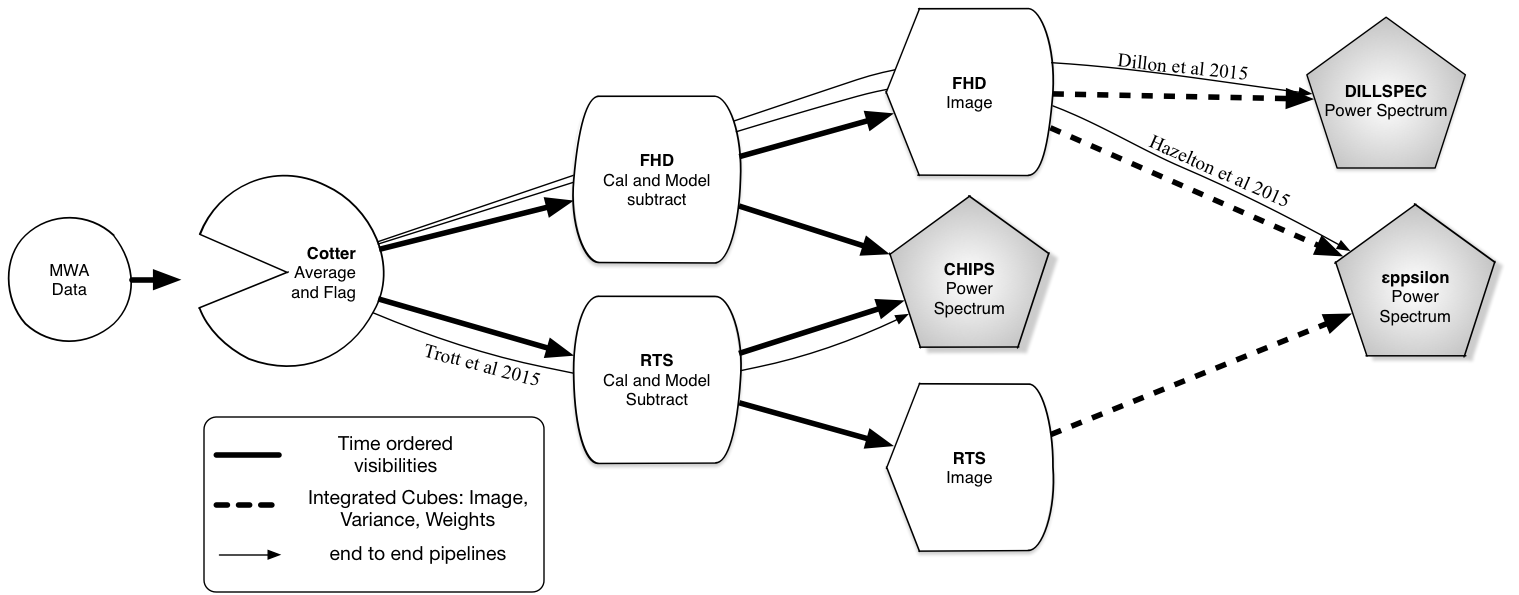
\includegraphics[width=\textwidth]{figures/MWA_Pipes.png}
\caption{Parallel pipelines with cross-connections after foreground subtraction and imaging are compared against each other. Pipelines used to reach the cited power spectrum results are indicated with thin lines; citations for each block are listed in Table \ref{tab:pipeline_cites}. Cotter uses AOFlagger to flag RFI and averages by a factor of 8. The averaged data are passed to either FHD or RTS for calibration, foreground subtraction and imaging. Both of these packages generate integrated residual spectral image cubes as well as matching cubes of weights and variances.  \eppsilon{} and \empirical{} use these cubes to estimate the power spectrum. Meanwhile, CHIPS taps into the RTS and FHD data stream to get calibrated and foreground-subtracted time-ordered  visibilities which it then grids with its own instrument model to estimate the power spectrum. 
}
\label{fig:pipes}
\end{center}
\end{figure*}

\subsection{Calibration and Imager \#1: RTS}
\label{sec:RTS}

The MWA Real Time System (RTS; \cite{Mitchell:2008p707,Ord:2010p8442}) was initially designed to make wide-field images in real time from the MWA 512-tile system \citep{Mitchell:2008p707}.  On the de-scoped 128 element array, it has been implemented as an offline system, where it has been adjusted to compensate for the lower filling factor \citep{Ord:2010p8442}.  The RTS incorporates algorithms intended to address a number of known challenges inherent to processing MWA data, including; wide-field imaging effects, direction-dependent (DD) antenna gains and polarization response, and ionospheric refraction of low-frequency radio waves. Each MWA observation (112s) is processed through a separate instance of the RTS. The RTS is also parallelized over frequency so that each coarse channel (1.28\,MHz broken into 40 kHz channels) is processed largely independently of the other coarse channels, with only information about peeled source offsets communicated between processing nodes.   

The RTS calibration strategy is based upon the `peeling' technique proposed by \cite{Noordam:2004p2379} and a foreground model using a cross-matching of heritage southern sky catalogs\footnote{See Table \ref{tab:cal_sub_parms}} with the MWA Commissioning Survey.  The cross-matching is done using the PUMA code which uses Bayesian inference to build a self-consistent set of SEDs for sources using data from catalogs with varying frequency and resolution. The brightest apparent calibrators in the field of view are sequentially and iteratively processed through a Calibrator Measurement Loop (CML). During each pass through the CML; i) the expected (model) visibilities of known catalog sources are subtracted from the observed visibilities. For the data processed in this work, 1000 sources are subtracted for each observation. ii) The model visibilites for the targeted source are added back in and phased to the catalog source location. Any ionospheric offset of the source can now be measured by fitting a phase ramp to the phased visibilities. iii) The strongest sources are now used to update the direction-dependent antenna gain terms, while weaker sources are only corrected for ionospheric offsets. For this work, 5 sources are used as full DD calibrators and 1000 sources are set as ionospheric calibrators. The CML is repeated until the gain and ionospheric fits converge to stable values. A single bandpass for each tile is found by fitting a 2nd order polynomial to each 1.28\,MHz-wide coarse channel. The $\sim$1000 strongest sources are then subtracted from the calibrated visibilities.   Calibration and model subtraction parameters are summarized in Table \ref{tab:cal_sub_parms}.  Model subtracted visibilities are passed to the RTS imager and to the CHIPS power spectrum estimator. %how much flux is subtracted in total?

The RTS imager uses a snapshot imaging approach to mitigate wide-field and direction-dependent polarization effects. Following calibration, the residual visibilities are first gridded to form instrumental polarization images which are co-planar with the array. These images are then regridded into the HEALpix \citep{Gorski:2005p7667} frame with wide-field corrections.  Weighted instrument polarization images are stored, along with weight images containing the Mueller matrix terms, so that further integration can be done outside of the RTS. It is also possible to use the fitted ionospheric calibrator offsets to apply a correction for ionospheric effects across the field during the regridding step or subtraction of catalog sources, but in this work this correction has not been applied. These snapshot data and weight cubes are then integrated in time to produce a single HEALpix cube. This cube, averaged over the spectrum, is shown, with and without foregrounds, in Figure \ref{fig:image_compare}.


\begin{deluxetable}{lll}
\tablecolumns{3}
\tabletypesize{\footnotesize}
\tablewidth{0pt} 
\tablecaption{MWA Reionization Calibration and Model subtraction Parameters. Counts are per-snapshot unless otherwise noted }
\tablehead{
\colhead{Parameter}  & 
\colhead{RTS} &
\colhead{FHD} 
}
\startdata
per cable passband & NA & 384 channels\tablenotemark{a}   \\
per antenna passband & 48 per tile\tablenotemark{b} & 3\tablenotemark{c}\\
per antenna gain & 2\tablenotemark{d} & 2\tablenotemark{d}  \\
peeling parameters & 4\tablenotemark{e} & None \\
peeled sources & 5 & None\\
subtraction catalog & Line\tablenotemark{f} & Carroll\tablenotemark{g} \\
number subtracted & 1000 & 6932 \\
\bf{Total free parameters} & \bf{6,420} & \bf{880} \\
\enddata
\tablenotetext{a}{for ea. of 6 cable types, averaged over 96 snapshots}
\tablenotetext{b}{2nd order polynomial per coarse channel}
\tablenotetext{c}{poly fit over full band, 2nd order for amp, 1st for phase}
\tablenotetext{d}{amplitude and phase}
\tablenotetext{e}{Direction Dependent (DD) gain fits}
\tablenotetext{f}{MWA Commissioning Survey\cite{Hurley-walker:2014p45},\cite[VLSSr]{2014MNRAS.440..327L},\cite[MRC]{Large:1991p7760},\cite[SUMSS]{Mauch:2003p8804},\cite[NVSS]{Condon:1998p7986},cross matched using PUMA (Line et al, in prep) \url{github.com/JLBLine/PUMA}}
\tablenotetext{g}{Combination catalog of legacy catalogs and sources deconvolved from this data (Carroll et al in prep)}
\label{tab:cal_sub_parms}
\end{deluxetable}



\subsection{Calibration and Imager \#2: FHD}
\label{sec:FHD}
Fast Holographic Deconvolution (FHD, \cite{Sullivan:2012p9457}) is a calibration and imaging algorithm designed for very wide field of view interferometers with direction- and antenna-dependent beam patterns. Variable beam patterns are used to grid visibilities to the $uv$ plane and its inverted operation for de-gridding simulations to form model visibilities, this careful accounting of weights provides a necessary accounting of information loss caused by the inherent size of the dipole element.

The FHD calibration pipeline generates a model data set, computes a calibration solution which minimizes the difference with the data, smooths the calibration solution to minimize the number of free parameters, and outputs the residual. The calibration model is formed from sources found by deconvolving, in broadband images, about 75 of the 96 snapshots included here and retains those which are common to all snapshots and pass other consistency checks (Carroll et. al. in prep). In each snapshot sources are included in the model if they are at or above 1\% of the peak primary beam, this amounts to about 7000 sources and a flux limit of about 80mJy with slight variations snapshot to snapshot. Most sources in this catalog have spectral indexes between 0 and -2 with the majority near a mean of $-0.8$, which corresponds to a 13\% difference across the 30\,MHz.  Spectral index is not directly modeled, spectra are simulated to be flat, however, during catalog subtraction, the data are multiplied by a positive spectral index of 0.8 such that most sources will appear to be flat. Full spectral modeling of catalog sources will be included in future analyses.


The goal of FHD's calibration is to minimize the number of free parameters with the twin goals of minimizing potential signal loss and in building a deep understanding of instrumental systematics. Here we give a brief description of the instrument model, a listing of all the parameters mentioned here is also given in Table \ref{tab:cal_sub_parms} along with a rough accounting for the total number of fitting parameters. Initial complex gain solutions computed using the Alternating Direction Implicit technique described in \citet{sal14} for each antenna, channel and polarization.  This generates a gain and phase for every channel on every tile, for each 112s snapshot.  Most antennas have similar solutions with the main features corresponding to the exact type and length of analog cable feed of which there are 6 different types; per-tile solutions are further averaged into per-cable-type and averaged over the entire 3 hour observation. After these solutions are divided out, the residual per-tile solutions are further fit for a second order amplitude spectral polynomial and a 1st order phase slope. This is done on every snapshot to account for temperature-driven amplifier gain changes. 
One systematic easily visible in the power spectra is a small reflection corresponding to the 150m cables. This is fit and removed as a phase delay with a $\sim$0.1dB amplitude in the time averaged per-tile bandpass solutions.


The residual time-ordered visibilites are then passed to CHIPS and to FHD imaging for formation of spectral cubes.  The FHD imager  produces snapshot cubes using the MWA beam model described by \cite{Sutinjo:2015RaSc...50...52S} and averaged in time. This image, averaged over the spectral dimension, is shown, with and without foregrounds, in Figure \ref{fig:image_compare}.

\subsection{Comparing Calibration and Imaging Steps}
\label{sec:comparing_imaging}
Through the parallel-but-convergent development of these imagers have emerged two very similar systems, however some differences remain in the analysis captured here. The two primary differences are in the treatment of calibration and in the subtracted catalogs.  

In both pipelines the calibration is a two step process. First, calibration solutions for each channel, and antenna are computed by solving for the least-squares difference with a model data set. Next, those solutions are fit to a model of the array; for example fitting a polynomial to the bandpass. FHD and RTS take different approaches to this step, a fact reflected in the the number of free parameters in this fit. A smaller number of parameters minimizes the possibility of cosmological signal loss; more free parameters can absorb physics missing from the instrument model.  As tabulated in Table \ref{tab:cal_sub_parms} the RTS fits for 6,420 free parameters while FHD fits for $\sim$880.  


In practice, some parameters will be averaged over more than a single night which will further reduce the number of free parameters per observation, though hundreds to thousands of free parameters is still typical. This is a large number but it is considerably smaller than the 180 million data points typically recorded in a two minute observation. 

As has been noted, there is nearly an order of magnitude difference in the number of free parameters, which is worth considering. The primary difference is in the treatment of the passband.  There are a number effects which show up in the passband calibration. The edges of the 1.28\,MHz bands are known to be subject to aliasing from adjacent coarse channels as well as under-sampling when cast to 4bit integers by the correlator (van Vleck corrections) and so are flagged. This flagging creates a regular sampling function which shows up as the characteristic horizontal lines in a 2D power spectrum. Added to this is a small amount of interference flagging.  Additionally, reflections at analog cable junctions show up as additional spectral ripple corresponding to the length of the cables.    

The RTS fits for a low order polynomial on every 1.28\,MHz chunk on every antenna, while FHD averages each channel over all antennas to get a common passband for all and then fits a low order polynomial to get any tile to tile variation. This significantly reduces the number of free parameters and the likelihood of signal loss, though leaving open the possibility of additional un-modeled instrumental effects.

%TODO add 
The construction of the foreground subtraction model is also a point of difference between the two pipelines.
As noted in Table \ref{tab:cal_sub_parms}, foreground/calibration models contain different numbers of sources which have been derived by different means. The RTS catalog cross-matches multiple heritage southern sky catalogs with the MWA Commissioning Survey using the Bayesian cross-matcher PUMA (Line et al in Prep).  The FHD subtraction model contains sources found in a deep deconvolution of this same data set. Both catalogs have the goal of producing a reliable set of sources that minimizes false positives and accurately reflects resolved components, though they go about it in different ways. The FHD catalog focuses on the reliability aspect by performing a deconvolution on every snapshot used in the observation and selecting sources which appear in most observations (Carroll et al, in prep). The RTS catalog has used the somewhat less precise MWA commissioning catalog but by cross-matching these sources against many other catalogs of known sources and fitting improved positions and fluxes, the accuracy is seen to increase.


\begin{figure*}[htb]
\begin{center}
\includegraphics[width=1\textwidth]{figures/FHD_RTS_image_compare.png}
\caption{A comparison between the image outputs of the FHD (left), RTS (center) and their difference (right) averaged in the spectral dimension and projected from native HEALpix to flat sky. The images have been left in the natural weighting used by image-based power spectrum schemes and no deconvolution has been applied.   In the top row, no foreground model has been subtracted; the residual shown represents a 15\% difference. On the bottom both have subtracted their best model of the sky containing similar sets of thousands of sources, most pixels the difference is 30\% or lower.   The difference between foreground subtracted images reveals a good agreement on large scale structure and small differences in the fluxes of a few sources.
%TODO this caption could be improved
\label{fig:image_compare}}
\end{center}
\end{figure*}


\subsection{Power Spectrum \#1: \eppsilon}
\label{sec:EPPSILON}
\eppsilon{} calculates a power spectrum estimate from image cubes and
directly propagates errors through the full analysis, see \eppsiloncite{} for a full description. The design criteria for this method is to make a relatively quick and uncomplicated estimate of the power spectrum to provide a quick turnaround diagnostic. The input to \eppsilon{} is gridded image cubes for  each 112s snapshot, such as are produced by FHD or RTS imaging, in which the data has been split into interleaved time samples (referred to as even and odd cubes) along with matched cubes containing the modeled instrumental weighting and variance. These snapshot HEALpix cubes are integrated in time keeping pixels with a beam weight of 1\% or more, a cut which effectively limits the field of view to $\sim$20\arcdeg. The accumulated data, weight and variance cubes are Fourier transformed along the two spatial dimensions into $uvf$ space, where the spatial covariance matrix is assumed to be diagonal. This is approximately true if the $uv$ pixel size is well matched to the primary beam size, so the  \eppsilon{} DFT grid size is restricted to being equal to the width of the FT primary beam; ie 1/(field of view). The data (variance) cubes are then divided by the weight cubes (weight cubes squared) to arrive at the best estimates of the sky and variances. Next the sum and difference of the even and odd cubes are computed with variances given by adding the reciprocal of the even and odd variances in quadrature. The difference cube then contains only noise (as long as the time interleaving is fine enough) and the sum cube contains both sky signal and noise.

The next step is to Fourier transform in the frequency direction. Here we choose to use the full 30\,MHz spectral window, weighted by a Blackman-Harris window function, which heavily down-weights the outer half of the band to effectively sample 15\,MHz; a cosmological redshift range of 0.86. This weighting scheme minimizes the covariance of bright foreground modes between power spectrum modes as described in \cite{Thyagarajan:2013p10039,Parsons:2012p8896,Vedantham:2012p9026}, among others.  The transform of the spectral dimension is done using the Lomb \& Scargle periodogram to minimize the effects of regular gaps in the spectrum which occur every 1.28\,MHz.    The sky signal power is  estimated by the square of the sum cube minus the square of the difference cube, which  is mathematically identical to the even/odd cross power if the even and odd variances are identical, while the square of the difference cube provides a realization of the noise power spectrum. Diagnostic power spectra are generated by averaging cylindrically to a two dimensional $k_{\|},k_{\bot}$ power spectrum.  These are shown in the left column of Figure \ref{fig:pspec_compare}.  One dimensional power spectra (shown in Figure \ref{fig:1D_pspecs}), are calculated by a similar process but only including the inner third of the spectrum (for a redshift range of 0.3) and then averaging along shells of constant $k$, masking points within the foreground wedge\footnote{Here defined, conservatively, as the light travel time across the baseline plus the delay associated with the pointing furthest from zenith. It is indicated as a solid line on Figure \ref{fig:pspec_compare}.} and weighting by variance.

%TODO 1D power spectra?





\subsection{Power Spectrum \#2: CHIPS}
\label{sec:CHIPS}
The CHIPS power spectrum estimation method computes the maximum likelihood estimate of the 21~cm power spectrum using an optimal quadratic estimator formalism and is more completely described in \chipscite{}.  The design criteria for this method were to fully account for instrumental and foreground induced covariance in the estimation of the power spectrum.  The approach is similar to that used by \cite{Liu:2011p8763}, but with the key difference of being performed entirely in $uvw$-space, where the data covariance matrix is simpler (block diagonal), and feasible to invert. This approach also allows straightforward estimation of the variances and covariances between sky modes by direct propagation of errors. CHIPS takes as input calibrated and foreground subtracted time-ordered visibilities. Tapping into the pipeline post-calibration but before imaging, CHIPS uses its own internal instrument model to estimate and propagate uncertainty.	

The method involves four major steps: (1) Grid and weight time-ordered visibility channels onto a $uvw$-cube using the primary beam model, (2) compute the least squares spectral (LSS) transform along the frequency dimension to obtain the best estimate of the line-of-sight spatial sky modes (this technique is comparable to that used by \eppsilon), (3) compute the maximum-likelihood estimate of the power spectrum, incorporating foregrounds and radiometric noise,  averaging $k_x$ and $k_y$ modes into annular modes on the sky, $k_\bot$; (4) compute the uncertainties and covariances between power estimates. The first step is the most computationally-intensive, requiring processing of all the measured data. The main departure point for CHIPS from \eppsilon{} is in the much finer resolution of the $uv$ grid.  Using an instrument model, CHIPS calculates the covariance between $uv$ samples as a function of frequency.  Since the beam and $uv$ sampling function are both highly chromatic, extra precision in this inversion is thought to be highly beneficial. After a line of sight transform similar to that used by \eppsilon{}, this covariance information is inverted to find the Fisher Information, the maximum likelihood power spectrum, and covariances between measurements.  The maximum likelihood estimate of the power in each $k_\bot,k_\parallel$ mode is shown in the right column of Figure \ref{fig:pspec_compare} and averaged in spherical bins in Figure \ref{fig:1D_pspecs}. This last averaging step includes an additional weighting by the known power spectrum of a confused foreground in a process described in more detail for these data by \chipscite{}. The power spectra shown in Figure \ref{fig:1D_pspecs} show an excess of power in excess of the expected noise. This excess is notably similar between both calibration/foreground subtraction pipelines. The amount of power in the excess, as compared with the error bars, also depends rather dramatically on the range of $k$ bins included in the final averaging to the 1D.  These are discussed in more detail in section \ref{sec:power_spectrum_comparison}.

\subsection{Power Spectrum \#3: Empirical Covariance}
\label{sec:empirical_cov}

The \empirical{} power-spectrum estimation method computes a 1D power spectrum using a quadratic estimator formalism. The method and its application to this data is described in more detail by \dilloncite{}.

The quadratic estimator method of \cite{Liu:2011p8763} treats foreground residuals in maps as a form of correlated noise and simultaneously downweights both noisy and foreground-dominated modes, keeping track of the extra variance they introduce into power spectrum estimates. This technique can be computationally demanding but using acceleration techniques described by \cite{Dillon:2013p10497}, has been applied to the previous MWA 32T results of \cite{Dillon:2014p9788} while a very similar technique, working on visibilities rather than maps, was used for the recent PAPER 64 results of \cite{2015ApJ...809...61A}.  \dilloncite{} build on these methods to mitigate errors introduced by imperfect mapmaking and instrument modeling through empirical covariance estimation, assuming all data covariance is sourced by foregrounds.

\empirical{} takes as input FHD calibrated images with foregrounds subtracted as well as possible, split into even and odd time-slices and averaged over many observations. From these cubes, it estimates the frequency-frequency foreground residual covariance in annuli in $uvf$ space, assuming that different uv cells have uncorrelated foreground residuals. This assumption, similar to that made by CHIPS, allows the combined foreground and noise covariance to be inverted directly. The resulting power spectrum is shown in Figure \ref{fig:1D_pspecs} for direct comparison with the CHIPS result. 



\subsection{Benefits of Comparison}
\label{sec:benefits_of_comparison}


One benefit from having multiple pipelines is the freedom to investigate  different optimization axes.  The design of the \eppsilon{} power spectrum estimator emphasizes speed and relative simplicity, choices  motivated by the need to understand the effect, on the power spectrum, of processing decisions such as observation protocol, flagging, and calibration. Using \eppsilon{} we have discovered and corrected multiple systematic effects, primarily those of a spectral nature which were not obvious in imaging but quite apparent in the 2D power spectrum. With the ability to quickly form power spectra on different sets of data, \eppsilon{} has been an important tool for selecting sets of high quality data. 

In contrast, CHIPS starts from time-ordered data and in its calculations emphasizes a more full accounting of instrumental and residual foreground covariance. Not only does this higher resolution covariance calculation provide a more accurate accounting of the instrumental window function on the power spectrum, but it also allows for more precise weighting schemes based on knowledge of the statistical properties of the residual foregrounds. This is useful when making 1D power spectra where foreground-like modes can be down-weighted in the average. 


\section{Comparison Discussion}
\label{sec:results}

Inspecting a comparison of the images and power spectra reveals several common features. Images before and after foreground subtraction are shown in Figure \ref{fig:image_compare}, presented in the natural weighting used by the power spectrum estimators without application of any further cleaning.  Putting the same 3 hours of MWA data into each pipeline, we inspect output images before and after foreground subtraction. The pre foreground-subtracted (sometimes called the ``dirty'' image) have residuals at about the 15\% level, after foreground subtraction the differences are somewhat larger at 30\%. Residuals in the dirty maps are largest  around bright sources. This is most likely due to slight differences in the calculation of image plane weights which are dramatically emphasized by the broad psf from the natural weighting. As evidenced by the clean residual maps, the point source subtraction is well modeled when subtracted in the visibilities.  The foreground subtracted images (sometimes called ``residual'' images) show a much closer agreement both around the subtracted sources and in the large scale structure. Large scale structure is more difficult to distinguish. Inspection of the snapshot images before averaging in time and frequency revealed that the structure is constant across both time and frequency, which suggests real Galactic emission rather than sidelobes or aliasing.  



\subsection{Power Spectra}
\label{sec:power_spectrum_comparison}
Application of our two independent power spectrum estimators to our two calibration and foreground subtraction pipes gives us a total of four different power spectra (Figures \ref{fig:pspec_compare} and \ref{fig:1d_kperp}).  Each power spectrum estimator has been developed to target the output from a ``primary'' calibration and foreground subtraction process --the diagonal elements of Figure \ref{fig:pspec_compare}-- and have been highly optimized to that up-stream source of data.  The off-diagonal power spectra were created using auxiliary links which import the data and the metadata produced by the foreground subtraction step.  Since they are less highly optimized, lacking as they do the advantage of a close working relationship, these pathways represent an upper limit on the variance to be expected from small analysis differences but allow us to look for effects common to foreground subtraction or to power spectrum method.


Properties shared by all are the large amount of power at low $k_{\parallel}$ roughly at an amplitude of $10^{15}$ mK$^2$/(Mpc/h)$^3$. This emission is approximately flat over most of $k_{\perp}$ but rises steeply rise at low $k_\perp$. The amplitude agreement is particularly apparent in Figure \ref{fig:1d_kperp}. A model of smooth galactic emission has not been subtracted which likely contributes to this steep rise. The ``wedge'' shaped linear dependance on baseline length in the 2D power spectra is due to the inherently chromatic response of a wide field instrument to smooth spectrum foregrounds; sources entering far from the phase center appear as bright pixels at higher $k_\parallel$ with sources on the horizon at the edge indicated by Figure \ref{fig:pspec_compare}'s  solid black line. The solid and dotted lines in the figure indicate the upper boundaries of power from sources at the horizon and at the beam half power point, respectively.  With the exception of some instrumental features foreground power is well isolated within this expected boundary. This emission is also visible in the image cubes as side-lobes extending from outside of the imaged area which move as function of frequency.  Observations recorded when the Galactic plane is near the horizon have a much larger wedge component and have been excluded from this analysis. See \cite{2015ApJ...804...14T} and \cite{2015ApJ...807L..28T} for a detailed discussion of the foreground contributions to the power spectra in this data. 

The two main instrumental systematics are horizontal striping due to missing or poorly calibrated data at the edges of regular coarse passbands and vertical striping due to spectral variation near uneven $uvf$ sampling. The former can be minimized by careful calibration of the passband, the latter by $uv$ rotation synthesis and by accounting for covariance between $uvf$ samples. 

The most noticeable difference between the different pipeline paths is in the power level in the window above the horizon and below the first coarse passband line (between 0.1 and 0.3 $k_\parallel$ and 0.01 and 0.05 $k_\perp$). FHD to \eppsilon{} displays a noise-like window in the 2D space, with a number of points dipping below zero while the other methods are noise like only at at much higher $k$s.  One commonality between all power spectra with this positive bias is a relatively higher amplitude of the coarse passband lines. 


The final analysis step is to average into 1D power spectra along shells of constant $k$. These are shown in Figure \ref{fig:1D_pspecs} for three of the four analysis tracks\footnote{The RTS$\to$\eppsilon{} spectrum is excluded here because image-plane uncertainties are not yet available as outputs from the RTS.} shown in Figure \ref{fig:pspec_compare} with the addition of the \dilloncite{} points and a theoretical sensitivity curve calculated using the 21CMSENSE sensitivity code\footnote{\url{github.com/jpober/21cmsense/}} by \cite{Pober:2014p10390}.

The positive biases visible in the 2D power spectra are also apparent here. Only a few a few points  are consistent with zero at 2$\sigma$, however most some are very close to the theoretical sensitivity curve and have errors matching those predicted for noise.
 The power spectra fall into two groups, those calculated from input image cubes (\eppsilon{} and \empirical{}) and those calculated directly from visibilities using CHIPS. The image-based points are somewhat deeper at low $k$, as noted in the 2D plots.  Points from CHIPS are biased more strongly at low $k$ but the slope is flatter and converges with the other pipelines at higher $k$.  

\subsection{CHIPS bias and the interpretation of error bars}
Part of the CHIPS bias is due to the calculation of weightings. Default CHIPS analysis uses a statistical model of confused foregrounds to down-weight biased modes, particularly those correlated with the wedge power. For this reason it is desirable to include the wedge modes in that 1D average. However it significantly changes the interpretation of error bars; points in which a significant amount of power have been down-weighted will have error bars much larger than thermal. In the interest of comparing with the other methods, these power spectra have been calculated using points only lying outside the wedge horizon. This limits the amount of wedge-to-window covariance CHIPS can remove and contributes to the larger bias. 

Including the full wedge in the CHIPS covariance calculation offers foreground suppression, but also introduces a foreground component into the error bars. Compare in Figure \ref{fig:CHIPS_compare} the RTS$\to$CHIPS power spectrum in Figure \ref{fig:1D_pspecs} with that given by \chipscite{} which used the same data shown here, though only 1/3 of the 30MHz band.  In both, CHIPS has down-weighted by a model of foreground covariance formed by propagating a statistical model of confused sources. The only difference is that black excludes the wedge but red does not. When the wedge is included the modeled foregrounds in those voxels dominate the covariance weights. Applying these weights essentially moves the foreground bias into the error bars and asserts that, given our best model of foregrounds, the power spectra are completely consistent with noise and  foregrounds.

The power spectra in Figure \ref{fig:1D_pspecs} show the range of results possible given the same input data. Though they do not all agree, they do paint a consistent picture.  Differences partly come from the definition of error bars but also indicate the relative difficulty of methods. Methods which rely on an imager seem to perform somewhat better. This is perhaps unsurprising. CHIPS computes the instrumental correlation matrix in visibility space using beam, bandpass, etc. As the CHIPS analysis exists entirely in the visibility space, errors in modeling the instrument model elements are perhaps more difficult to detect than they are in the image space.  However, we do not suggest that visibility-based calculations like CHIPS are doomed to failure; rather the opposite. The instrument models will continue to improve, and this improvement will be easily validated by comparison with the other pipelines.






\begin{figure*}[htbp]
\begin{center}
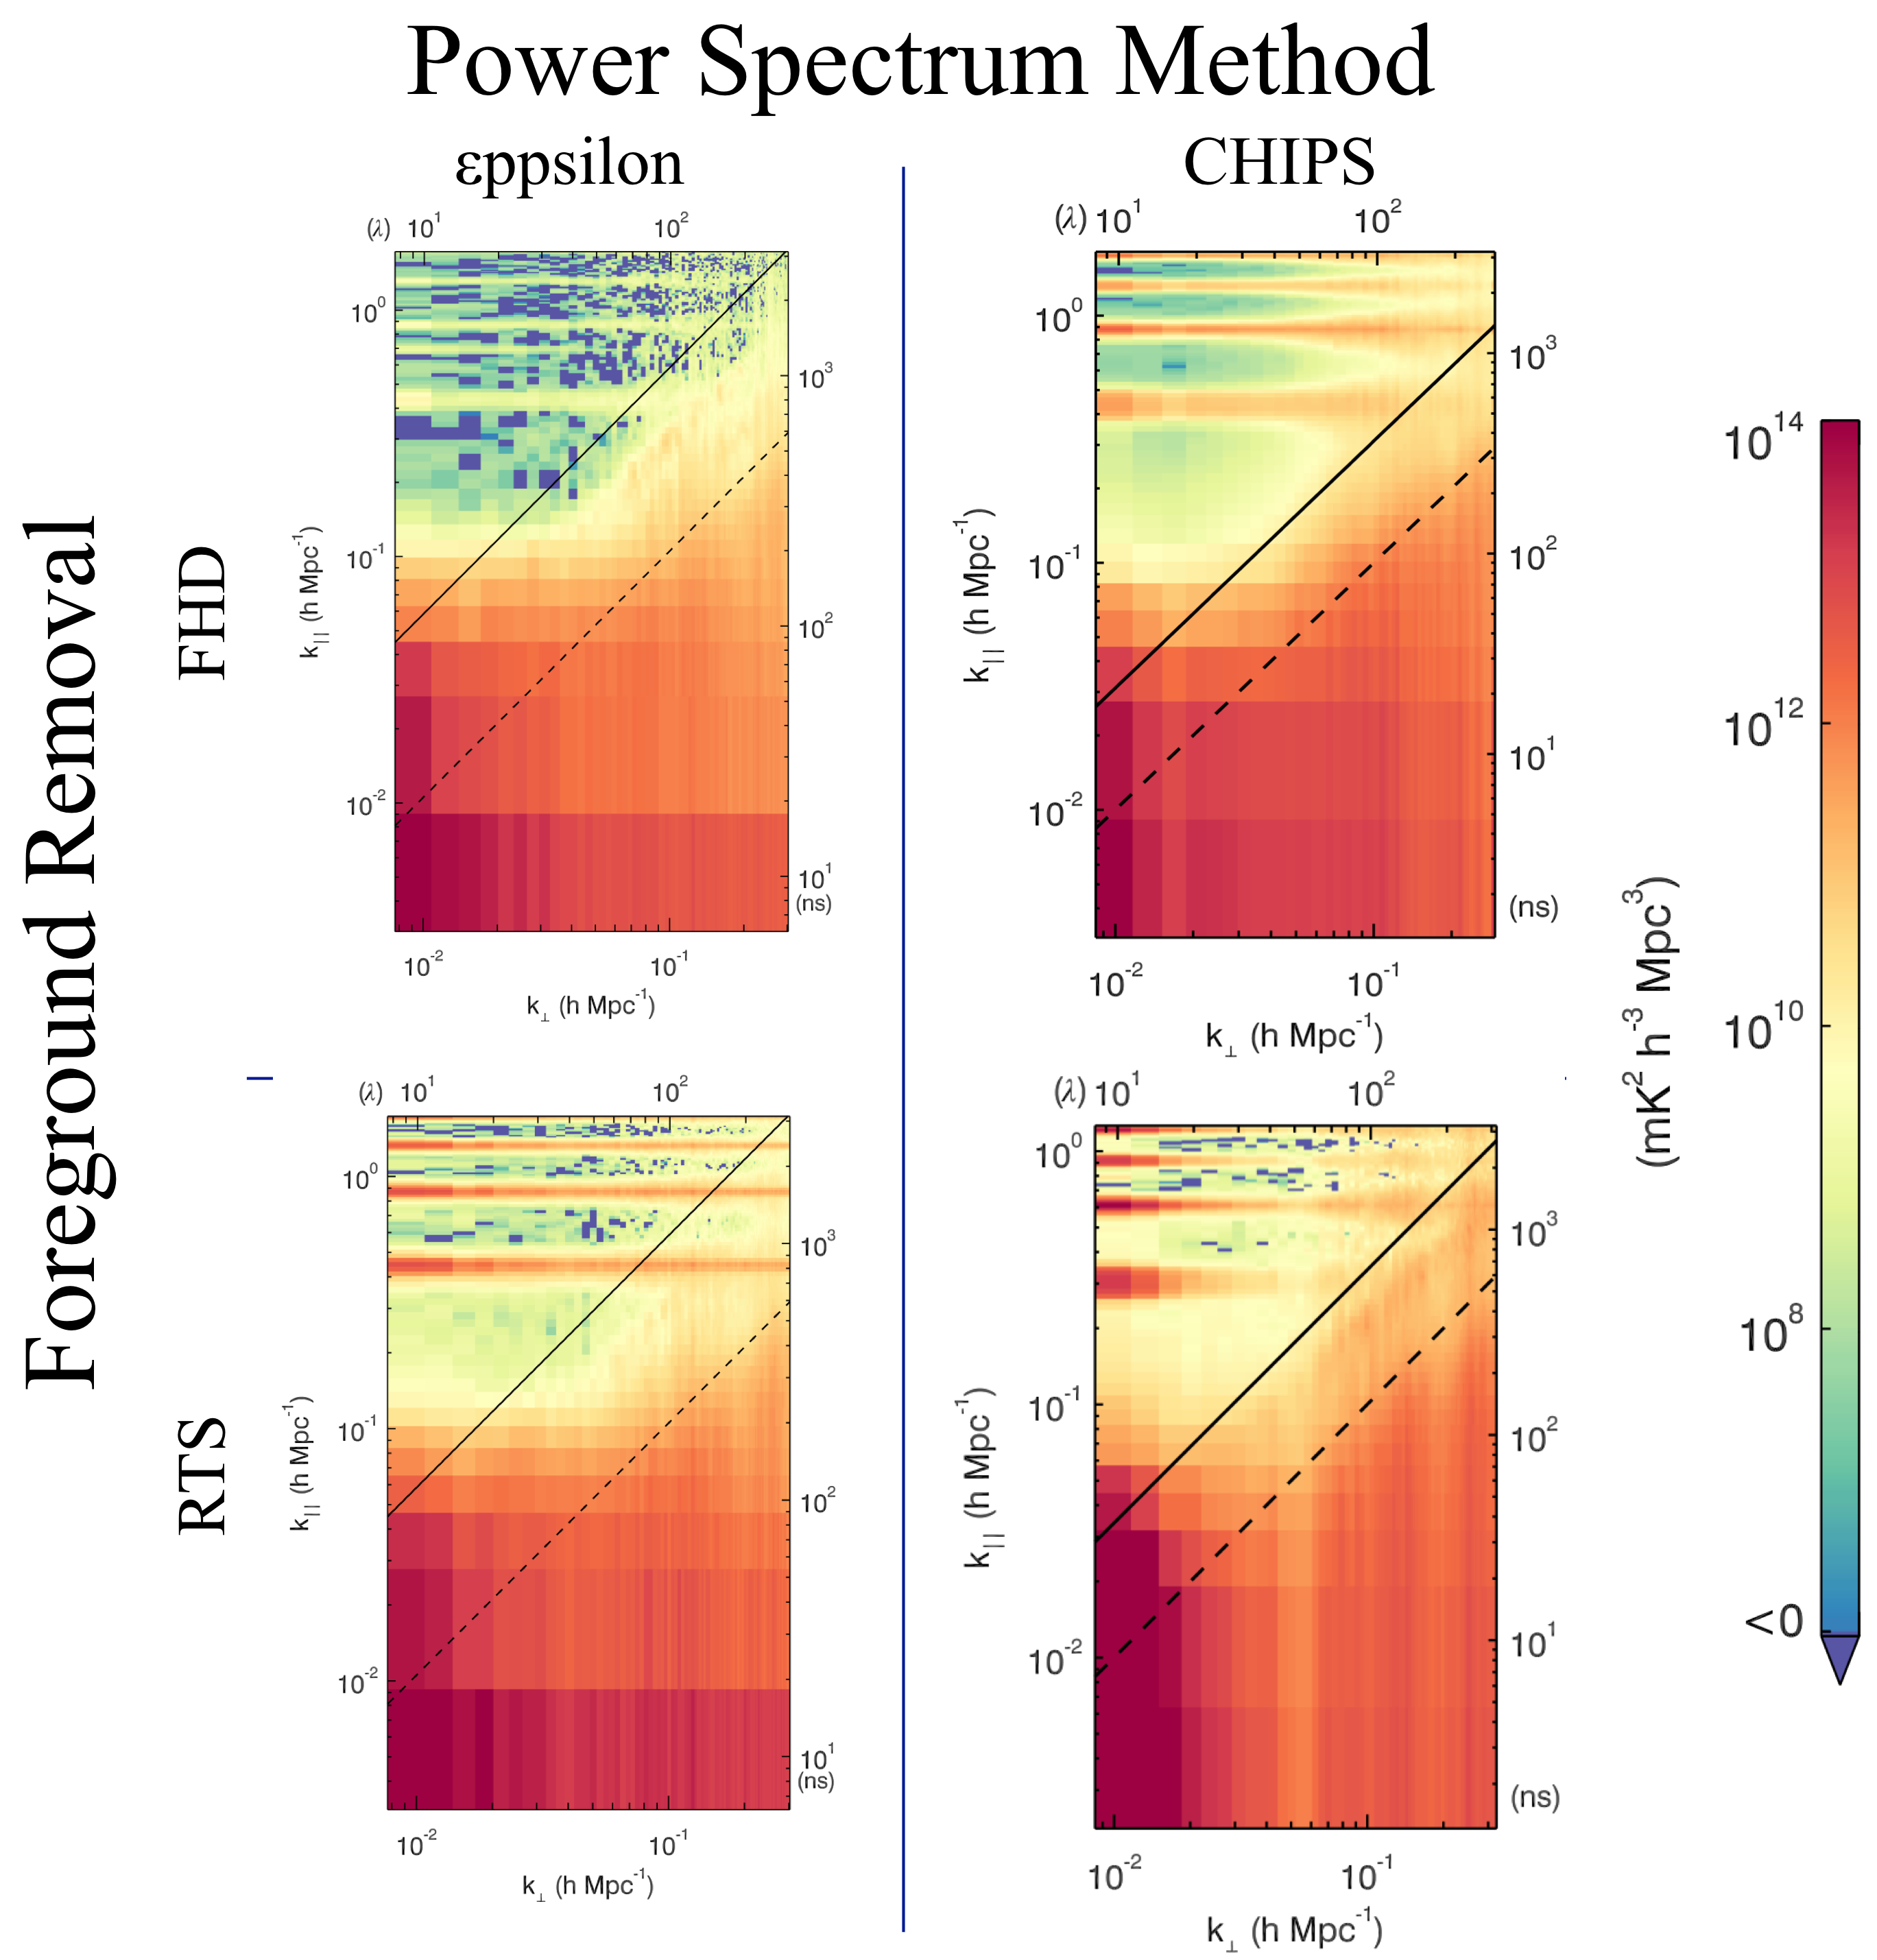
\includegraphics[width=0.8\textwidth]{figures/MWA_PS_compare/MWA_PS_compare.png}
\caption{Power spectra computed using two foreground subtraction methods and two power spectrum estimation methods on the data shown in Figure \ref{fig:image_compare}; the power spectrum has been computed in 3D spectral line cubes and then averaged cylindrically.  In the top row data have been calibrated and foreground subtracted using the Fast Holographic Deconvolution method, in the bottom row by the MWA Real Time System.  In the left column, power spectra have been estimated with \eppsilon{}, which emphasizes speed and full error propagation, in the right column, CHIPS corrects more correlation between $k$ modes.  All spectra display the now well-understood ``wedge''-shaped foreground residual and horizontal stripes caused by evenly spaced gaps in the instrument pass-band. Because all the power spectra are calculated by cross-multiplying independent data samples, measurement noise remains zero mean; negative regions are therefore indicative of noise-dominated regions.   \label{fig:pspec_compare}}
\end{center}
\end{figure*}
%TODO include Josh's 2D?

\begin{figure}[htbp]
\begin{center}
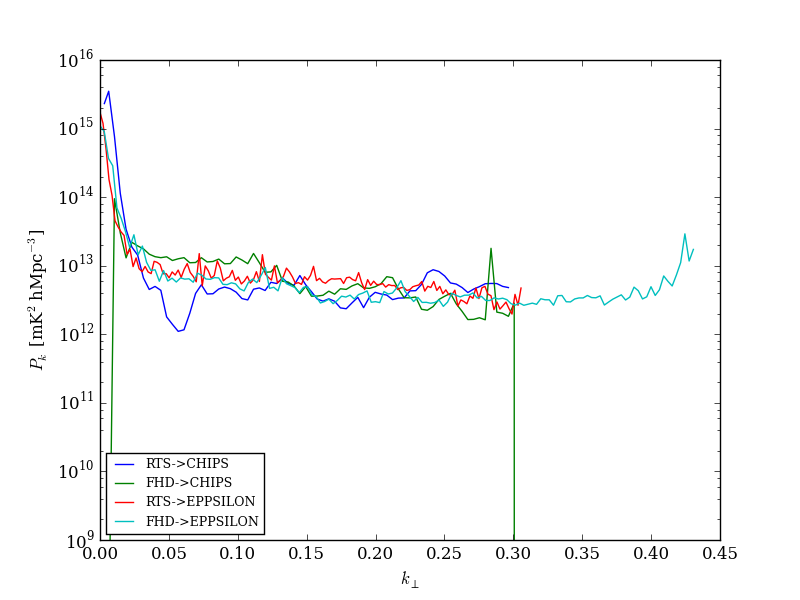
\includegraphics[width=0.5\textwidth]{figures/MWAPipeline_compare_1d_kperp.png}
\caption{Horizontal cut sampling the $k_\parallel = 0$ mode of the 2D power spectra shown in Figure \ref{fig:pspec_compare} indicating good agreement on flux scale and foreground power shape over most k modes. The foreground subtraction model only includes point sources. The steep rise is likely due to the bright, smooth galactic foreground emission visible in the residual images in Figure \ref{fig:image_compare} and power spectra by \cite{2015ApJ...807L..28T}.}
\label{fig:1d_kperp}
\end{center}
\end{figure}


\begin{figure*}[htbp]

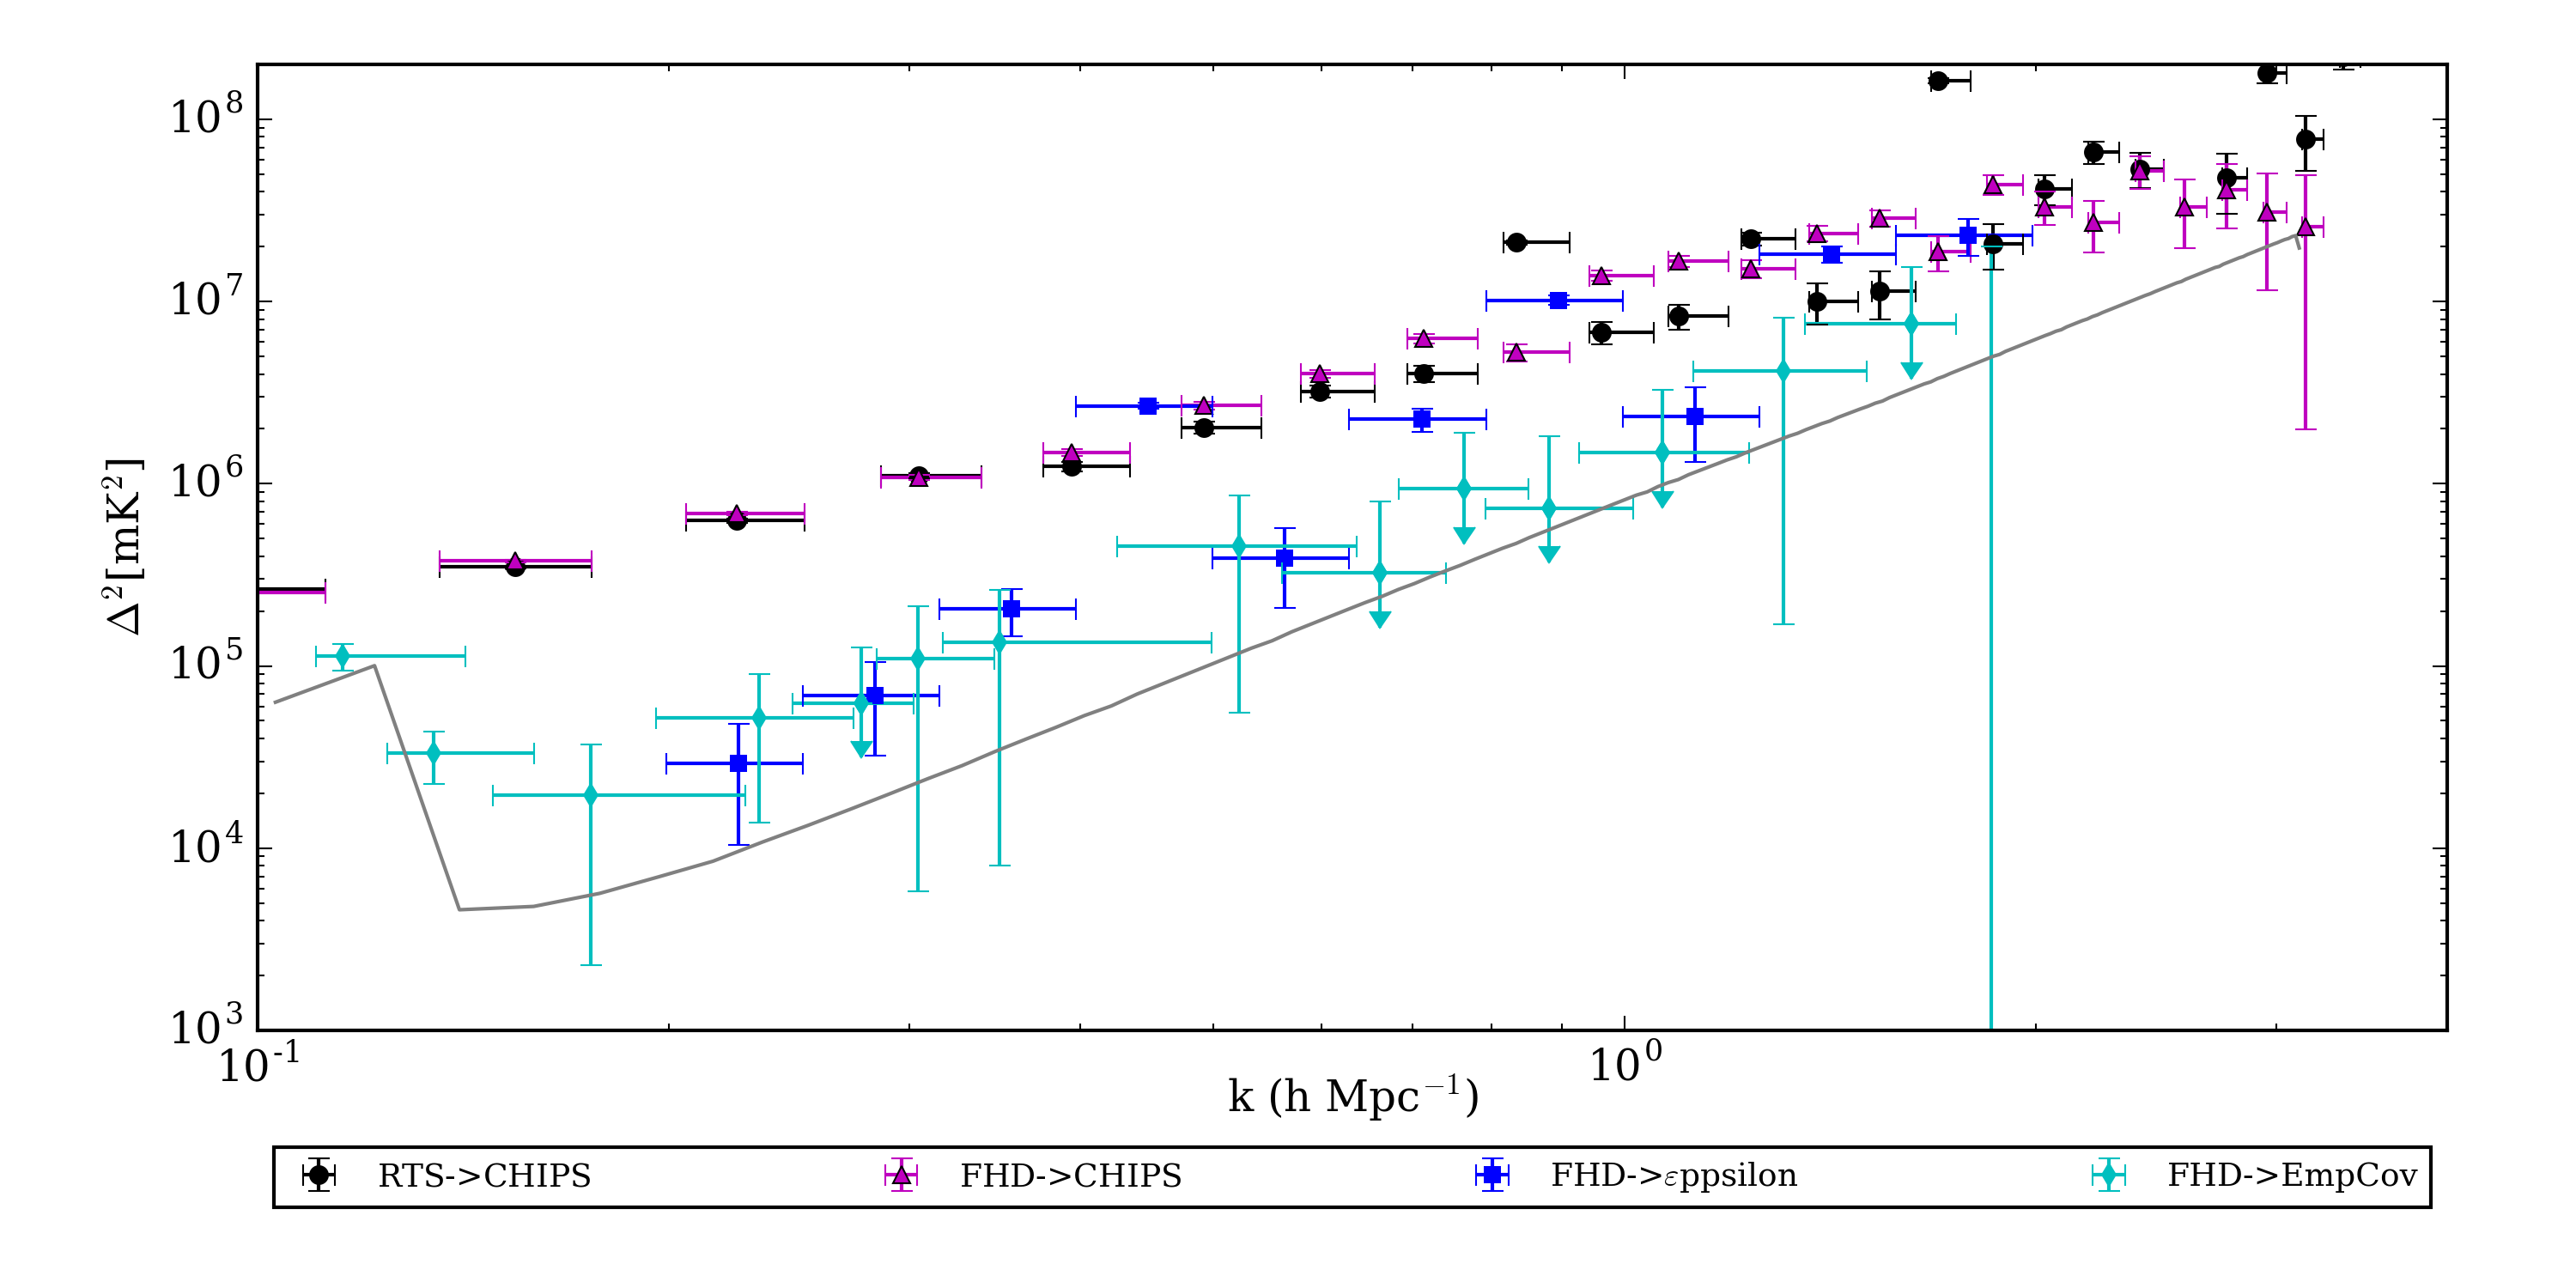
\includegraphics[width=\textwidth]{figures/MWA_PS_Compare/MWAPipeline_compare_1d_radial_logbryna.png}
\caption{Power spectra averaged along shells of constant $|k|$ with 2$\sigma$ errors. In three hours of data, four different methods demonstrate different kinds of limits on the power spectrum. Note that of the four pathways shown in Figure \ref{fig:pspec_compare}, only three are included here, but we have now included the power spectrum from \dilloncite{}. The \eppsilon power spectra of RTS outputs are excluded because error bars are not available. Many of the features visible in the 2D plots are also visible here: the excess in the CHIPS spectra is clearly visible as is a smaller excess in the \eppsilon{} spectrum.  The black line indicates 2$\sigma$ bounds for points dominated by noise.  Power levels for typical theoretical models are typically in the 5 to 10 mK$^2$ range across these $k$ modes.
\label{fig:1D_pspecs}}

\end{figure*}

\begin{figure*}[htbp]
\begin{center}
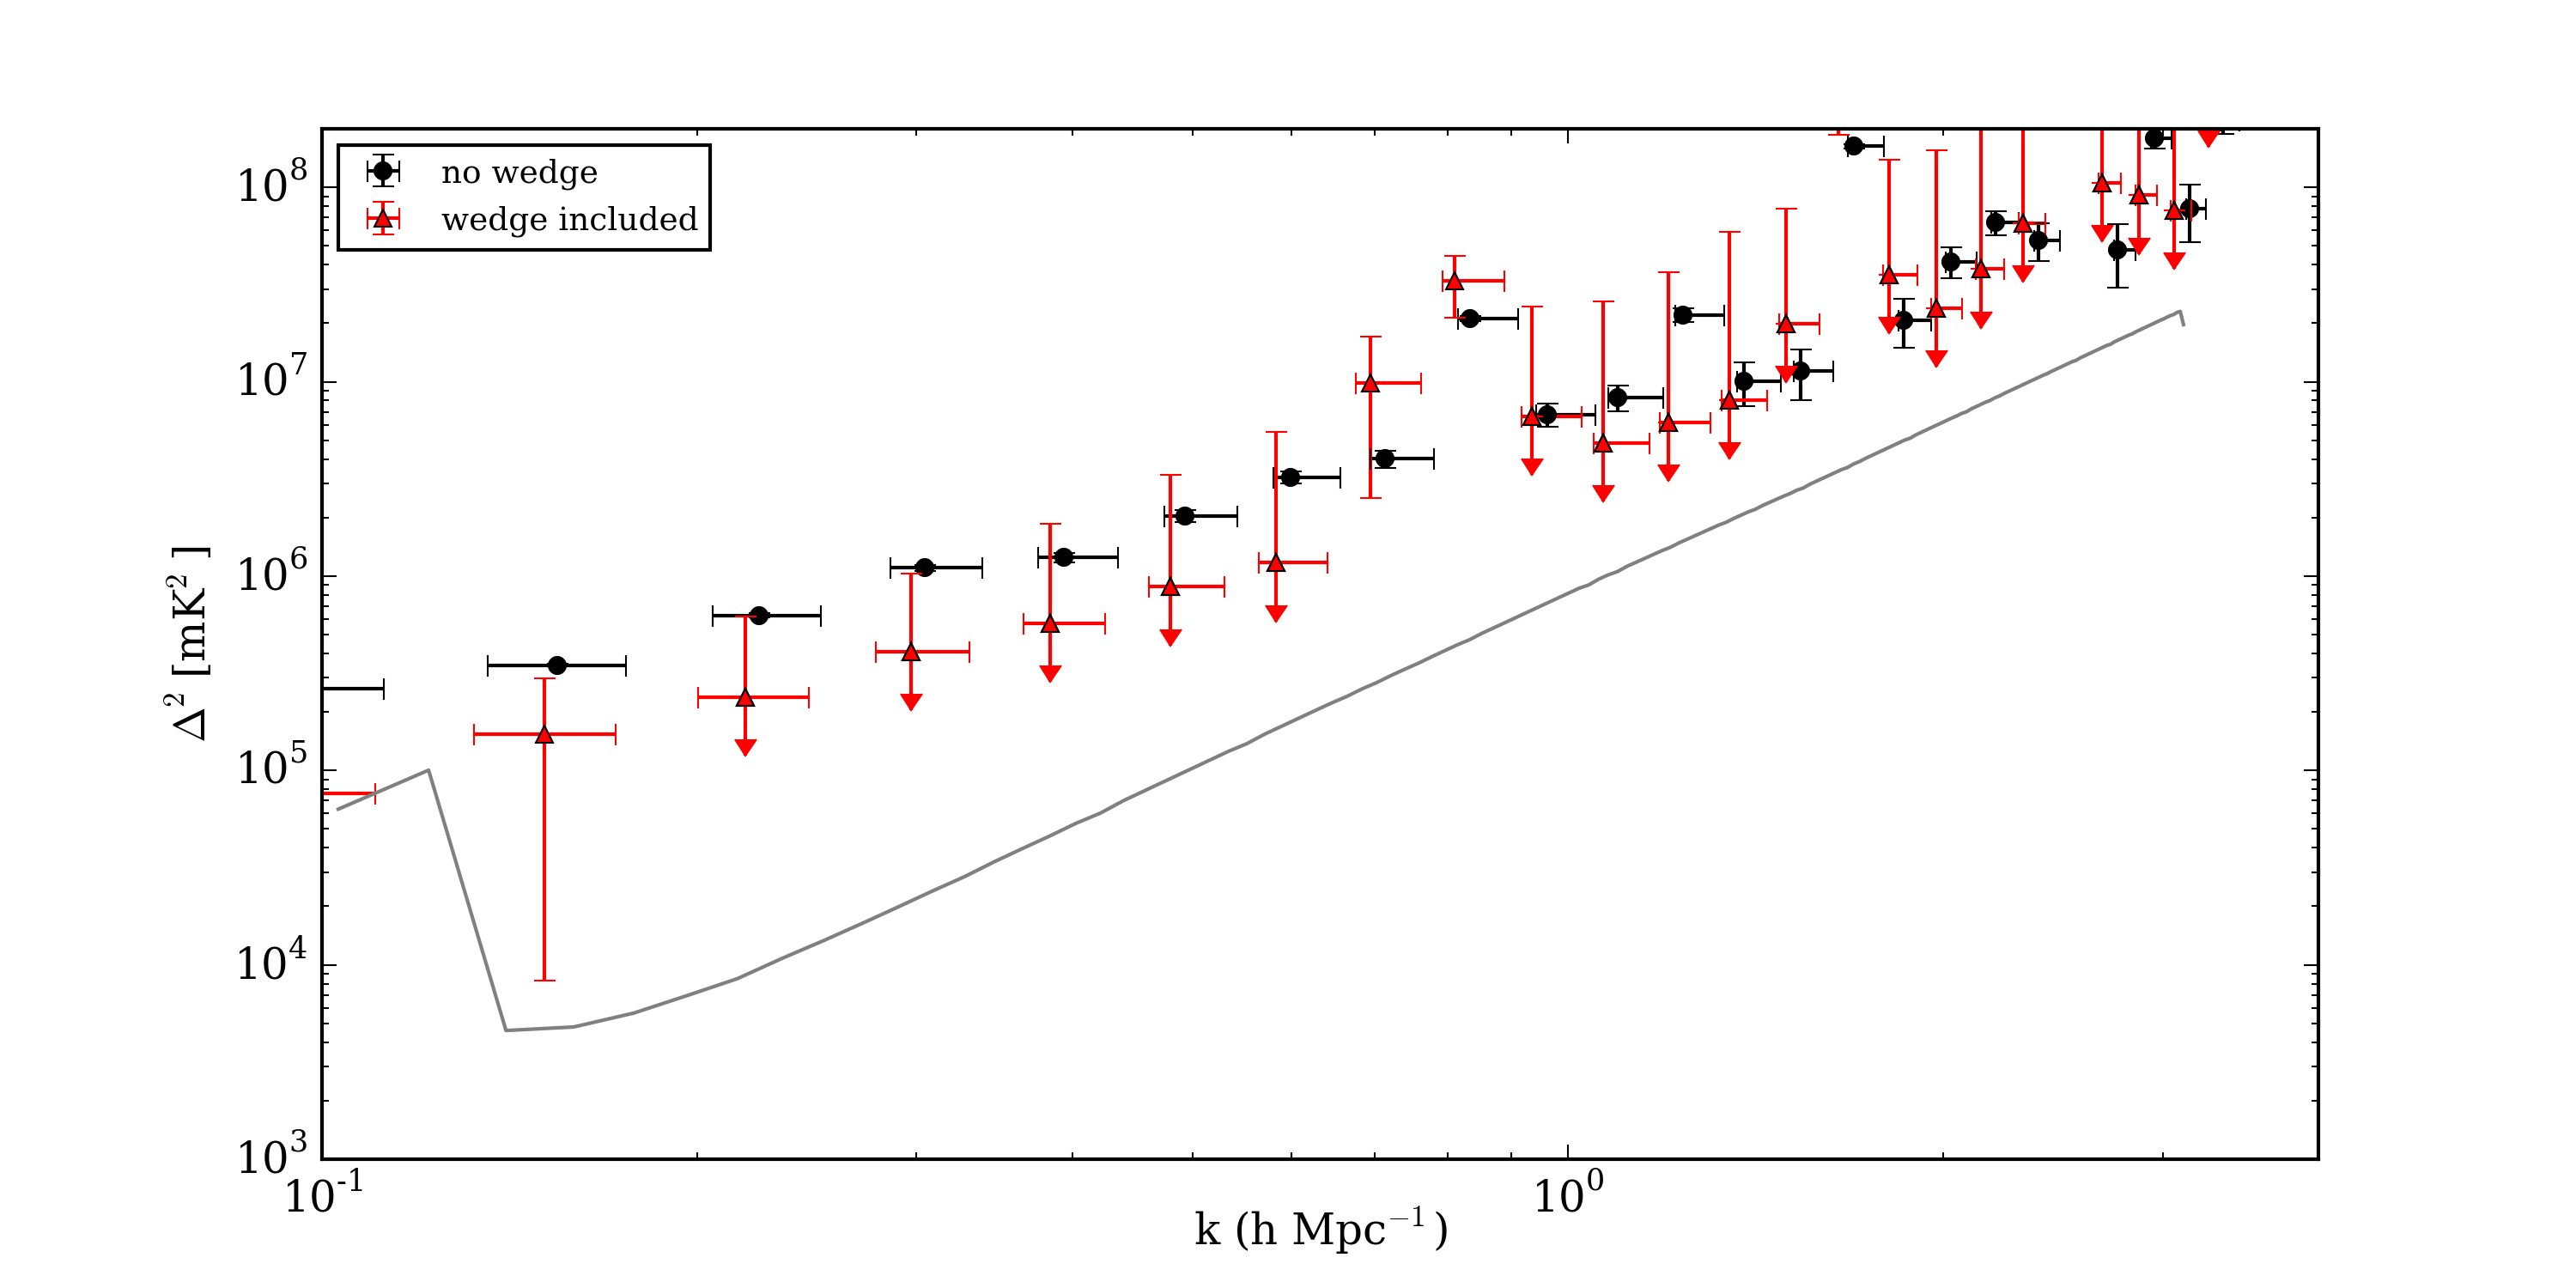
\includegraphics[width=\textwidth]{figures/MWA_PS_Compare/MWAPipeline_compare_1d_radial_chips_pub.png}
\caption{An example of the dramatic impact that weighting and covariance minimization has on the interpretation of error bars.  Here we compare the RTS$\to$CHIPS power spectrum from Figure \ref{fig:1D_pspecs} with that given by \chipscite{}. The latter was made with the same data but only 1/3 of the 30MHz band, and so slightly higher error bars.  In both, CHIPS downweights by a model of foreground covariance formed by propagating a statistical model of confused sources. The only difference is that black excludes the wedge but red does not. When the wedge is included the modeled foregrounds in those $k$-space voxels dominate the covariance weights. Applying these weights essentially moves the foreground bias into the error bars and asserts that, given our best model of foregrounds, the power spectra are completely consistent with noise and foregrounds and do not provide evidence for a significant cosmological 21 cm signal.}
\label{fig:CHIPS_compare}
\end{center}
\end{figure*}

\section{Lessons from Comparing Independent Pipelines}
\label{sec:lessons}
          A data analysis pipeline is necessarily built on a complex software framework which is only imperfectly described in prose and is susceptible to human error.  Comparison between independently developed analysis paths, each with their own strengths and limitations, is essential to placing believable constraints on the Epoch of Reionization. The ongoing comparison between independent MWA pipelines has revealed a number of issues both systematic (related to our understanding of the instrument or foregrounds) and algorithmic (optimizing our use of this knowledge) which we will briefly mention here.
      
\begin{itemize}

\item \emph{ Systematic example: cable reflections}

As discussed above, one significant difference between the two pipelines is the number of free parameters fit in the calibration step, particularly in the spectral dimension.  Both calibration pipelines begin by calibrating each channel and then averaging over a number of axes.  The RTS fits a low order polynomial, piecewise, to each of the 24 1.28MHz sub-band solutions, while FHD fits a similar order polynomial to the entire  band's calibration solution.  Inspection of power spectra calibrated using the FHD scheme revealed previously unknown spectral features corresponding to reflections on the analog cables at the -20dB level (~1.5\%). FHD calibration now includes a fit for these reflections and the feature is substantially reduced. These features are fully covered by the RTS fit (which uses of order 10 times as many free parameters as FHD). 

\item \emph{Calibration example: number of sources}

In early comparisons between RTS and FHD images one immediately apparent difference was the somewhat lower dynamic range of the RTS images.  This was traced to the largest (at the time) difference between the two approaches; RTS used the more traditional radio astronomy practice of calibrating to a pointing on a bright source at the beginning of each night and then transferring the calibration to the rest of the observations, whereas FHD was calibrating against the foreground model using the cataloged sources within the field of view (a few thousand). This dramatically highlighted the breakdown of approaches designed for traditional dish telescopes with a narrow field of view.  The MWA field of view is so wide, that even the calibration pointing included many sources of brightness comparable to the calibrator. These sources were not included in the calibration model and thus limited the accuracy of the calibration. Also, owing to the phased array beam steering, the primary beam for the calibrator pointing is very different from the beams used for the primary reionization observations, particularly in polarization response.  So, though the instrument itself is highly stable in time over many hours, calibrations must be carefully matched up with the observing parameters or experience a dramatic loss of imaging dynamic range, both spatially and spectrally. The addition of ``in field'' calibration, where the foreground subtraction model is also the calibration model, significantly improved the RTS images and brought the two imagers into substantial agreement. 


\item \emph{Algorithmic example: full forward modeling for absolute calibration and signal loss}

During the comparison process, one way in which all pipeline results differed from each other is in the overall amplitude of the power spectrum scale. Flux calibration, weightings, Fourier conventions and signal loss must all be well understood for good agreement to be reached.  Signal loss, in particular, must be examined closely. Unintentional or unavoidable down-weighting or subtraction of reionization signal could occur at multiple stages such as bandpass calibration, $uvf$ gridding, or inverse covariance weighting. These effects are best calibrated via forward modeling of simulated sky inputs. and in the process provides verification of the overall power spectrum scale.  For example, detailed simulations of reionization signals through FHD and \eppsilon{} found that in areas of dense $uv$ sampling, simulated power spectra experienced a 50\% reduction of detected power \eppsiloncite{}.  These simulated reionization data sets have been calibrated internally by comparing outputs at every step of the imaging and power spectrum process, and so are well understood at a detailed level, and suitable for use calibration standards for new pipelines.



\item \emph{Algorithmic example: w-planes in power spectrum calculation}


Many of the differences found between power spectra during the comparison were traced to the post-foreground-subtraction steps, particularly the implementation of new imaging and power spectrum estimation codes.  One example was an anomalous loss of power in CHIPS power spectra which particularly effected longer baselines.  CHIPS grids in a coordinate space defined by the baseline vector $\vec{b}$ and spectral mode $\eta$ and then uses an instrument model to diagonalize and sum in this sparse power spectrum space.  Unlike FHD which uses snapshots to avoid directly handling the third or `w' term of the baseline vector, CHIPS accumulates the entire observation into a full uvw$\eta$ hyper-cube.  The number and size of the voxels in this space, particularly in the w direction is a somewhat free parameter and relates to the precision of the instrument model, the amount of time included and other factors.  Subsequent, more detailed foreground simulations suggested a factor of 4 w resolution increase which eliminated the signal loss and dramatically improved agreement.


\item \emph{Interchange standards}

Finally, in the interest of transparency, we offer a somewhat prosaic but perhaps vital lesson regarding  nomenclature. For fixed dipole arrays there are (at least) two popular and mutually exclusive traditions. Tradition A: In keeping with the customary abscissa of latitude longitude plots, the east-west oriented dipole is labeled X.  Tradition B: Astronomically, the X polarization is measured as the amplitude of a dipole aligned with lines of constant Right Ascension; which for a source at zenith maps to north-south. We humbly suggest that those pursuing a cross comparison effort select one standard at the outset.  

\end{itemize}






  We must stress that without the ability to compare between independent pipelines, most of these effects would have gone un-detected or mis-diagnosed as algorithmic deficiencies and have persisted into the final result or motivated additional fitting parameters resulting in higher signal loss as well as a vague disquiet. In addition to pipeline redundancy, forward modeling can provide some important checks, for example the absolute calibration of FHD and \eppsilon{} described in \eppsiloncite{}, however the result is only as good as the model itself.
  
\section{Conclusions}
\label{sec:conclusion}
In this overview paper we have provided a top level view of foreground subtraction and power spectrum estimation methods of the MWA Epoch of Reionization project, described more completely in companion papers \eppsiloncite{}, \chipscite{}, and \dilloncite{}.  In this comparison we see that both foreground subtraction methods are able to reliably remove similar amounts of power.  Differences between the images are smaller than the remaining residual foregrounds by a factor of 3.2, suggesting an overall $\sim$30\% error on the aggregate calibration, foreground subtraction and imaging between the two pipelines.  The power spectra of these foreground subtracted outputs agree on the scale and distribution of power, though with some differences in the leakage of power into the window. These differences are partly due to definition of error bars and whether they include just noise or also foreground terms.  

Including foregrounds in the error calculation is a key exercise because it lets us answer more nuanced questions. Rather than simply: is the data inconsistent with a 21cm detection in the presence of noise? With CHIPS we can ask: Is the data inconsistent with a 21cm detection in the presence of noise and an a-priori foreground model? With \empirical{} we can ask: is the data inconsistent with a 21 cm detection in the presence of noise and a foreground model fit to the data? These are all good questions.

21cm cosmology experiments have very wide fields of view, dense samplings, drift scanning observing and the reionization science levies a requirement for very high, 10,000:1, spectral dynamic range. All of this has necessitated the development of new algorithms for calibration and imaging, as well as the surrounding scaffolding to process thousands of hours of data to achieve this precision.  This paper is the first step towards validating these pipelines and providing robust repeatable results.





\acknowledgments

This work was supported	 by the U. S. National Science Foundation (NSF) through award AST--1109257. DCJ is supported by an NSF Astronomy and Astrophysics Postdoctoral Fellowship under award AST--1401708. JCP is supported by an NSF Astronomy and Astrophysics Fellowship under award AST-1302774. CMT is supported by an Australian Research Council DECRA Award, DE140100316. This scientific work makes use of the Murchison Radio-astronomy Observatory, operated by CSIRO. We acknowledge the Wajarri Yamatji people as the traditional owners of the Observatory site. Support for the MWA comes from the U.S. National Science Foundation (grants  AST-1410484, AST-0821321, AST-0457585, PHY-0835713, CAREER-0847753, and AST-0908884), the Australian Research Council (LIEF grants LE0775621 and LE0882938), the U.S. Air Force Office of Scientific Research (grant FA9550-0510247), MIT School of Science, the Marble Astrophysics Fund, and the Centre for All-sky Astrophysics (an Australian Research Council Centre of Excellence funded by grant CE110001020). Support is also provided by the Smithsonian Astrophysical Observatory, the MIT School of Science, the Raman Research Institute, the Australian National University, and the Victoria University of Wellington (via grant MED-E1799 from the New Zealand Ministry of Economic Development and an IBM Shared University Research Grant). The Australian Federal government provides additional support via the Commonwealth Scientific and Industrial Research Organisation (CSIRO), National Collaborative Research Infrastructure Strategy, Education Investment Fund, and the Australia India Strategic Research Fund, and Astronomy Australia Limited, under contract to Curtin University. We acknowledge the iVEC Petabyte Data Store, the Initiative in Innovative Computing and the CUDA Center for Excellence sponsored by NVIDIA at Harvard University, and the International Centre for Radio Astronomy Research (ICRAR), a Joint Venture of Curtin University and The University of Western Australia, funded by the Western Australian State government.

\bibliography{library}

\end{document}
